% -*-coding: utf-8-*-

\documentclass[annotation,times]{itmo-student-thesis}

\graphicspath{ {../Images/} }
\usepackage{placeins}
\usepackage{algpseudocode}
\usepackage{hyperref}
\hypersetup{linktocpage}

\addbibresource{thesis.bib}

\begin{document}

\studygroup{4537}
\title{Построение семейств оптимальных маршрутов на морских картах}
\author{Громаковский И.Е.}
\supervisor{Ковалев А.С.}
\supervisordegree{магистр прикладной математики и информатики, начальник отдела, ЗАО «Кронштадт Технологии»}
\publishyear{2015}

\researchdirections{Целью настоящей работы является разработка программного модуля, решающего в режиме реального времени задачу поиска семейств оптимальных маршрутов кораблей на морских картах. Под семейством оптимальных маршрутов понимается множество маршрутов между начальной и целевой точкой, отличающихся способом обхода существенных препятствий.}

\researchpart{Для предобработки карт с целью получения графа были использованы методы вычислительной геометрии. Для поиска маршрутов были разработаны эвристики для обновления весов в графе и провеки критериев похожести маршрутов. С помощью различных оптимизаций удалось добиться работы в режиме реального времени.}

\economicpart{С помощью разработанного программного модуля капитаны кораблей могут более эффективно прокладывать маршруты, что может быть экономически выгодно.}

\ecologypart{Данная работа не оказывает влияния на вопросы экологии и не требует соблюдения никаких особых техник безопасности.}

\cwpublications{Данная работа не является продолжением курсовых работ, публикаций на её основе нет.}

\practicalimplications{Предложенный алгоритм был реализован и в настоящее время входит в состав программного обеспечения ЗАО «Кронштадт Технологии». Рекомендуется использование для решения задач поддержки принятия решения в навигационно-тактических системах морского назначения.}

\makebachelortitle

\tableofcontents

\startthechapters
% -*-coding: utf-8-*-
\startprefacepage

Задача поиска кратчайшего пути при наличии полигональных препятствий
хорошо известна и исследована. Классический способ решения этой задачи
описан в~\cite{de2000computational}. Одним из её практических
применений является поиск кратчайшего маршрута кораблей на морских
картах, то есть кратчайшего пути между двумя точками, проходящего по
воде. Однако при нахождении единственного кратчайшего маршрута
возникают различные проблемы.

Во-первых, кратчайший путь не всегда является действительно
оптимальным, с точки зрения пользователя. Например, на пути могут быть
каналы, проплыть через которые возможно только за большую плату, что
сделает такой маршрут менее привлекательным, чем какой-то другой,
более длинный маршрут. В каких-то местах может быть нежелательно
плавать по политическим соображениям, также у капитана корабля могут
личные предпочтения. Формализовать всё множество критериев,
описывающих оптимальность маршрута, едва ли представляется возможным.

Во-вторых, иногда может возникнуть ситуация, при которой
воспользоваться кратчайшим маршрутом не представляется возможным.
Например, где-то могут проходить военные учения, из-за чего движение
судов в таких местах будет запрещено. Информация, заложенная в карту,
по которой строился маршрут, могла устареть, и какая-то река или канал
могли полностью высохнуть. В таком случае пользователю хочется иметь
альтернативный маршрут.

В-третьих, иногда нужно направить большое количество кораблей из одной
точки в другую. Если сотни кораблей пойдут одним маршрутом, то они
могут потратить очень много времени в очереди, чтобы проплыть по
какому-нибудь каналу. Если же корабли пустить разными маршрутами, то
суммарные временные затраты могут быть существенно уменьшены, несмотря
на то что часть кораблей поплывёт не по кратчайшему пути.

Таким образом, возникает задача поиска семейств маршрутов между двумя
точками. При этом маршруты должны быть в некотором смысле оптимальны.
Например, логично требовать, чтобы маршруты были несильно длиннее
кратчайшего пути и попарно непохожи. Непохожие маршруты должны
отличаться способом обхода существенных препятствий. Сама по себе
данная задача не приводит к конечному результату, а лишь осуществляет
поддержу для принятия решения. Окончательное решение принимается
пользователем в голове, поэтому основное требование к задачам
поддержки принятия решения состоит в том, что они должны решаться
практически моментально, в режиме реального времени, чтобы не сбивать
пользователя с мыслей.

Для задачи поиска нескольких маршрутов (multipath planning) также
известны некоторые решения. Например, существуют различные алгоритмы
решения задачи $K$-shortest paths, состоящей в поиске первых $K$ путей
в графе по возрастанию длины~\cite{eppstein1998finding,
yen1971finding}. Однако нетрудно понять, что обычно такие пути будут
иметь много общих рёбер и проходить через одни и те же водоёмы. Также
известны и другие алгоритмы multipath planning~\cite{lim2005shortest,
dial1971probabilistic, mafast}. Например,
алгоритм~\cite{lim2005shortest} находит пути, которые имеют как можно
меньше общих рёбер, однако при его применении к имеющейся задаче
получаются похожие маршруты. Это связано с тем, что если есть, скажем,
два маршрута, один из которых проходит на километр южнее другого, то
они, как правило, хоть и почти не имеют общих рёбер, по сути являются
очень похожими, поскольку обходят все препятствия с одной стороны
(пусть и на разном расстоянии).

В первой главе приведён подробный обзор предметной области и
существующих алгоритмов, формализована постановка задачи.
Во второй главе описано теоретическое решение поставленной задачи,
рассмотрены вопросы предобработки исходных данных и поиска семейств
маршрутов. В третьей главе рассмотрены вопросы эффективной реализации
предложенного решения и приведены основные результаты работы.

\FloatBarrier


%-*-coding: utf-8-*-
\chapter{Обзор предметной области}

\FloatBarrier
\section{Планирование путей}

\emph{Планирование путей (англ. path planning, motion planning)} ---
область computer science, решающая задачу поиска пути из одной точки в
другую, удовлетворяющего некоторым ограничениям. В основе
планирования путей лежат такие науки, как вычислительная геометрия
и теория графов. В данной работе рассматривается планирование
маршрутов по воде по всему миру. В этом случае суша представляет из
себя полигональные препятствия. Как известно (TODO: сослаться), любой
кратчайший путь между двумя вершинами при наличии полигональных препятствий
представляет собой ломаную, вершины которой --- вершины полигонов. В
дальнейшем в данной работе слова «\emph{маршрут}» и «\emph{путь}»
будут использованы взаимозаменяемо.

\emph{Граф видимости (англ. visibility graph)} --- граф, вершины
которого являются вершинами полигональных препятствий, а ребро между
вершинами $u$ и $v$ принадлежит графу тогда и только тогда, когда
отрезок $uv$ не пересекает ни одно препятствие.

Таким образом, любой кратчайший путь между двумя точками является
кратчайшим путём в графе видимости и может быть найден, например, с
помощью алгоритма Дейкстры. Однако граф видимости, построенный по
контурам суши со всего мира, взятым с мелкомасштабной карты, содержит
слишком много рёбер, из-за чего поиск может выполняться довольно
длительное время. В связи с этим возникает другая задача: найти
маршрут, близкий к кратчайшему. Для этой задачи необязательно строить
граф видимости, достаточно ограничиться навигационным графом.

\emph{Навигационный граф} --- граф, построенный по полигональным
препятствиям, вершины которого соответствуют некоторым точкам в
пространстве, а ребро между вершинами $u$ и $v$ может принадлежать графу только
тогда, когда отрезок $uv$ не пересекает ни одно препятствие.

\FloatBarrier
\section{Планирование мультипутей}

\emph{Планирование мультипутей (англ. multipath planning)} ---
область computer science, решающая задачу поиска нескольких путей из
одной точки в другую, таких что каждый путь удовлетворяет некоторым
ограничениям, и при этом на множеством путей также наложены
ограничения. Например, задача поиска $k$ кратчайших путей через
полигональные препятствия.

При поиске единственного маршрута (например, кратчайшего по какой-либо
метрике) могут возникнуть следующие проблемы:
\begin{enumerate}
    \item Критерии оптимальности не всегда очевидны и формализуемы.
      Чаще всего интересует кратчайший маршрут, но иногда может быть
      нужен, например, самый экономный маршрут, который не обязан
      совпадать с кратчайшим. Также могут быть и другие критерии, в
      том числе составные, которые едва ли представляется возможным
      описать какой-либо метрикой. Например, вряд ли возможно
      формализовать политические факторы или личные предпочтения пользователя.
    \item Ненадёжность. Возможна ситуация, когда находится
      единственный маршрут, но воспользоваться им не представляется
      возможным. Например, в каком-то месте может быть временный
      запрет или просто слишком мелко. В таком случае требуется
      запасной вариант.
    \item Повышенная загруженность. Если приложение, находящее ровно
      один маршрут, набирает популярность, это может привести к тому,
      что некоторыми маршрутами будут очень активно пользоваться, что
      приведёт к повышенной загруженности. Например, одна компания
      может направить большое число судов из одной точки в другую.
      Если все они пойдут через один и тот же канал, то могут потерять
      крайне много времени.
\end{enumerate}

Известны различные алгоритмы поиска нескольких маршрутов, более
подробный обзор которых будет приведён во второй главе.

\FloatBarrier
\section{Постановка задачи}

В данной работе требуется исследовать вопросы планирования
мультипутей на морских картах. Для этого прежде всего требуется
наложить ограничения на множество находимых маршрутов, тем самым
определив понятие семейства оптимальных маршрутов. Следующий этап
состоит в исследовании имеющихся алгоритмов планирования мультипутей
для выяснения их применимости к поиску маршрутов по воде. Затем
требуется разработать и реализовать новый алгоритм, находящий
семейство оптимальных маршрутов. Необходимо, чтобы алгоритм работал в
режиме реального времени, затрачивая меньше секунды на запрос.

\FloatBarrier
\section{Семейство оптимальных маршрутов}

При поиске нескольких маршрутов в первую очередь возникает вопрос о
том, каким условиям должно удовлетворять результирующее множество
маршрутов. Разумеется, маршруты не должны быть похожи. TODO

\FloatBarrier


%-*-coding: utf-8-*-
\chapter{Теоретическое решение}

\label{ch:theoretical-solution}

\section{Предобработка данных}

\label{sec:preprocessing}

Для решения поставленной задачи первым делом необходимо построить
навигационный граф. Подразумевается, что карта содержит множество
контуров, которые можно классифицировать на ограничивающие воду и
ограничивающие сушу. Контура заданы как последовательности точек в
плоской проекции Меркатора~\cite{thomas1952conformal}. Для построения
графа выполняется определённый набор действий.

Первым делом происходит упрощение водных контуров, полученных из карты, и
объединение их в один полигон. Упрощение выполняется по двум причинам:
\begin{itemize}
    \item Хоть такая модификация и может повлиять на корректность
      маршрута, действительно сильно некорректных маршрутов от неё
      появиться не может. Неформальная постановка задачи допускает
      такие модификации. Кроме того, планируется искать маршруты по
      всему земному шару, поэтому мелкомасштабные детали не несут
      никакой информации.
    \item Данные с мелкомасштабной морской карты содержат слишком
      много точек, из-за чего в навигационном графе будет крайне много
      вершин и рёбер, если не упрощать контура. Это приведёт к тому,
      что граф будет занимать слишком много памяти, а поиск путей в
      нём будет занимать слишком много времени.
\end{itemize}
Для упрощения используется алгоритм Дугласа-Пекера~\cite{douglas1973algorithms}.

После построения единого полигона, описывающего контуры воды, для него
строится straight~skeleton~\cite{aichholzer1996straight}, с помощью
которого выполняется смещение полигона внутрь. Это делается по
следующим причинам:
\begin{itemize}
    \item Корабли, как правило, не плавают слишком близко к суше (в
      двенадцатимильной зоне)~\cite{o1984international}. При этом стоит
      отметить, что в данной задаче не требуется искать кратчайший
      маршрут, а требуется получать естественные маршруты, которые
      потенциально могут использоваться для реальных кораблей.
    \item Маршруты, проходящие по границе суши, хуже визуализируются,
      поскольку перемешиваются с сушей. В то же время при визуализации
      маршрутов, проходящих на небольшом расстоянии от суши, таких
      проблем не возникает.
    \item Такая модификация нейтрализует возможные нарушения
      корректности маршрута, возникающие из-за упрощения контуров.
      Если при упрощении любая точка смещается на расстояние не больше
      $l$, а смещение контура происходит на расстояние $d > l$, то про
      любую точку, принадлежащую итоговому полигону, можно сказать,
      что в исходной карте она точно принадлежит контуру с водой.
\end{itemize}

По смещённому полигону строится навигационный граф. Для этого на
плоскости, на которую спроецирована карта,
строится сетка с некоторым постоянным шагом. Для каждого ребра сетки
проверяется принадлежность полигону, ограничивающему воду. Если ребро
полностью принадлежит полигону, то оно добавляется в граф (вместе с
инцидентным вершинами). Помимо этого в граф добавляются все вершины
полигона и рёбра до видимых вершин (то есть рёбра, полностью
принадлежащие полигону) в некотором радиусе. При этом важно ограничить
максимальную длину ребра. Это связано с тем, что граф строится по
полигону в плоской проекции, и проверка принадлежности отрезка
полигону выполняется на плоскости. В то же время кратчайшее расстояние
между двумя точками на Земле достигается не для отрезка, а для дуги.
Поэтому такая проверка, вообще говоря, некорректна. Однако, если
ограничить длину ребра, то отклонение дуги от отрезка будет невелико.
Учитывая то, что полигон смещён внутрь, можно утверждать, что любое
ребро действительно будет проходить по воде, не пересекая препятствия.

Также в полученный граф добавляются дополнительные рёбра. Во-первых,
поскольку граф строится по контурам в проекции Меркатора, то в нём
отсутствуют рёбра через 180-ый меридиан. Такие рёбра добавляются в
граф. Во-вторых, добавляются рёбра, получившиеся в результате
«схлопывания» контуров полигона при построении straight skeleton'а.
Это необходимо сделать, потому что при смещении полигона некоторые
контура «схлопываются», объединяясь в один. Если между ними был,
скажем, какой-нибудь канал, то по нему нельзя будет пройти в итоговом
графе. Именно поэтому такие рёбра из straight skeleton'а добавляются в
граф. При этом они объединяются в цепочки рёбер, и к каждой цепочке
применяется упрощение с помощью модифицированного алгоритма
Дугласа-Пекера. Модификация состоит в проверке корректности
получающегося отрезка по исходному полигону.

\FloatBarrier

\section{Поиск одного маршрута}

\label{sec:single-search}

Прежде чем перейти к описанию алгоритма поиска семейств маршрутов,
необходимо детально описать процесс поиска одного маршрута в
построенном навигационном графе. Первым делом для двух заданных точек
проверяется принадлежность полигону, ограничивающему воду. Если точки
действительно находятся на воде, то по имеющейся сетке для них
находятся ближайшие вершины графа, и все корректные рёбра до ближайших
вершин добавляются в граф. После этого используется алгоритм
Дейкстры~\cite{dijkstra1959note} для поиска кратчайшего пути в графе между
этими двумя вершинами. Поиск останавливается, когда кратчайший путь до
нужной вершины найден.

Поскольку найденный путь не является действительно кратчайшим
маршрутом между двумя точками, производится попытка его сократить. Для
каждой вершины пути проверяется, можно ли её убрать из маршрута, не
нарушив его корректность и не увеличив длину пути. Если можно, то
такая вершина убирается из маршрута. Этот процесс может повторяться
несколько раз, для чего каждый отрезок пути разбивается на подотрезки
меньшей длины. После этого опять производится попытка выкинуть точки.
И так далее. Ещё одна модификация маршрута вызвана тем, что в связи со
структурой графа в маршруте могут появляться слишком острые углы (если
в каком-нибудь контуре, образованном при смещении полигона, есть
острый угол). В реальных маршрутах не бывает острых углов, поэтому
выполняется сглаживание маршрута, то есть замена острого угла ломаной,
аппроксимирующей дугу эллипса. При этом корректность такой замены
проверяется по исходному полигону, не смещённому внутрь.

\begin{figure}
    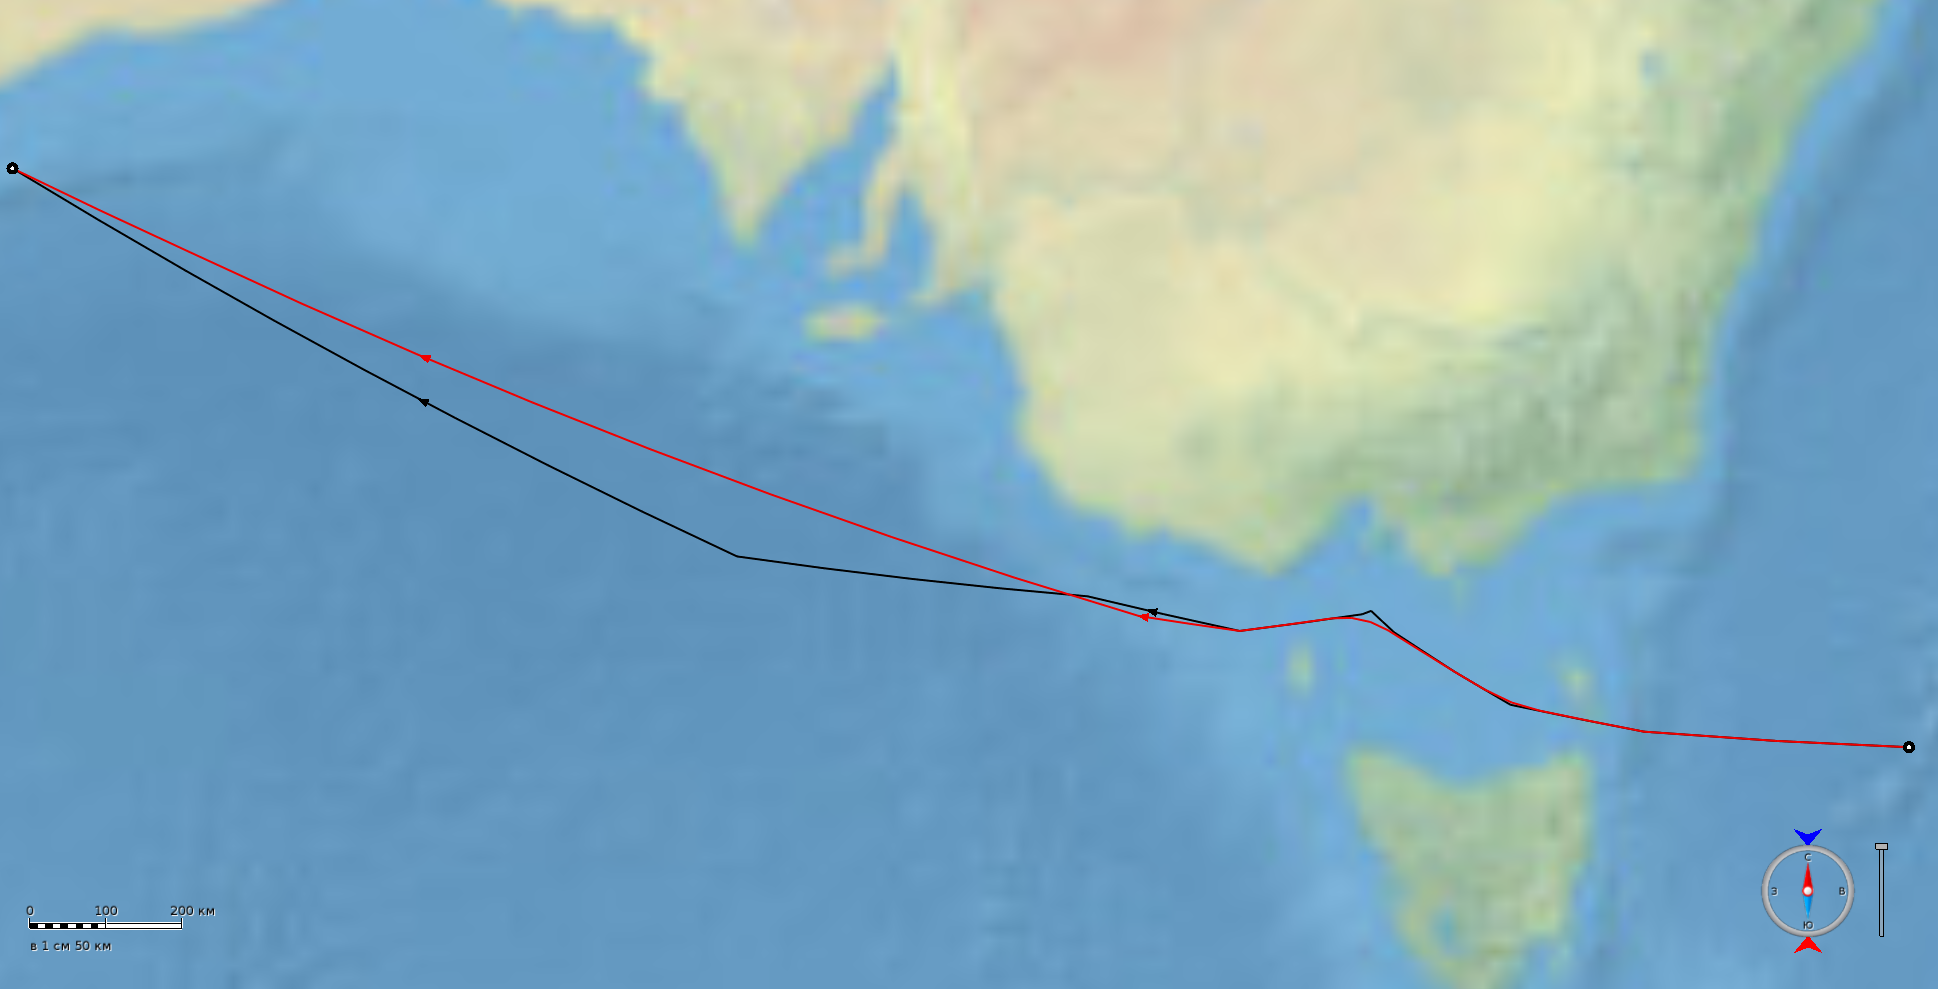
\includegraphics[width=\textwidth]{Solution/shortcut-and-smoothing}
    \caption{Сокращение и сглаживание маршрута}
    \label{fig:path-improvements}
\end{figure}

На рисунке \ref{fig:path-improvements} продемонстрирован эффект от
сокращения и сглаживания маршрута. Чёрной линией изображён кратчайший
путь в графе, а красной --- итоговый маршрут. Нетрудно видеть, что
левая часть маршрута сократилась, а в правой части произошло
сглаживание, что сделало маршрут более естественным.

\FloatBarrier

\section{Поиск нескольких маршрутов}

\label{sec:multi-search}

Для поиска нескольких маршрутов используется итеративный алгоритм. На
листинге \ref{alg:multipath} представлен псевдокод алгоритма. Первым
делом выполняется поиск первого маршрута описанным выше способом,
найденный маршрут добавляется в результирующее множество, запоминается
его длина. Затем, пока количество найденных маршрутов не достигнет
максимально возможного, выполняются следующие действия: обновление
весов рёбер в графе, поиск очередного маршрута, проверка критерия
остановки. Критерий остановки был сформулирован в формальной
постановке задачи и состоит в том, что длина найденного маршрута
должна быть не более чем в $C_0$ раз больше длины кратчайшего
маршрута, и не один из имеющихся маршрутов не должен быть похожий на
последний найденный. Функция $similar(p, q)$ проверяет, похожи ли
маршруты в соответствии с формализацией, приведённой в постановке
задачи. Практическая реализация этой функции описана в следующей
главе.

Остановимся поподробней на процессе обновления весов. Обновление весов
основано на введении для каждой вершины графа некоторого потенциала.
Чем больше потенциал вершины, тем сильнее увеличиваются веса
инцидентных ей рёбер. Чем ближе вершина к найденному маршруту, тем
сильнее должен увеличиваться вес инцидентных ей рёбер, чтобы
находились непохожие маршруты. Для поиска потенциалов первым делом
строится граф с фиктивной вершиной, из которой проводятся рёбра
нулевого веса во все вершины очередного пути (функция
$graph\_with\_fake$ в псевдокоде). Вводится максимальное расстояние,
равное $\frac{len}{C_1}$, где константа $C_1$ является параметром
алгоритма. Для всех вершин, до которых длина кратчайшего пути в графе
меньше этого расстояния, могут быть увеличины потенциалы. После этого
используется алгоритм Дейкстры для поиска кратчайших расстояний из
фиктивной вершины, при этом поиск заканчивается, когда достигнуто
максимальное расстояние (функция $shortest\_in\_radius$ в псевдокоде).
Кратчайшее расстояние до непосещённых вершин принимается равным
максимальному. Следующий вопрос состоит в вычислении потенциалов
вершин по найденным расстояниям и обновлении весов рёбер по введённым
потенциалам. Наиболее очевидным и простым решением является вычислять
значение потенциала, используя убывающую линейную функцию от
кратчайшего расстояния (например, $\frac{limit - dist}{A}$, где
$limit$ --- введённое выше максимальное расстояние, $dist$ ---
найденное кратчайшее расстояние от фиктивной вершины, $A > 0$ ---
некоторая константа), и прибавлять к весу ребра среднее арифметическое
потенциалов инцидентных ему вершин. Однако такой подход обладает
определённым недостатком.

\begin{algorithm}[!h]
    \begin{algorithmic}
        \Function{find\_paths}{}
            \State p, len $\gets$ find\_path()
            \State paths $\gets$ \{p\}
            \State min\_len $\gets$ len
            \While{paths.size() < max\_paths\_count}
                \State update\_weigths(p, len)
                \State p, len $\gets$ find\_path()
                \If{$len > C_0 \cdot min\_len$}
                    \State \Return paths
                \EndIf
                \For{q in paths}:
                    \If{similar(p, q)}
                        \State \Return paths
                    \EndIf
                \EndFor

                \State paths.insert(p)
           \EndWhile
        \EndFunction

        \Function{update\_weights}{p, len}
            \State g' $\gets$ graph\_with\_fake(p)
            \State limit $\gets \frac{len}{C_1}$
            \State d $\gets$ shortest\_in\_radius(g', fake, limit)
            \ForAll{v in p}
                \State d[v] = $\frac{limit}{M}$
            \EndFor
            \ForAll{v in vertices}
                \State potential = $1 + (max\_potential - 1) \cdot \frac{limit - d[v]}{limit}$
                \State potentials[v] = max(potentials[v], potential)
            \EndFor
            \ForAll{e in edges}
                \State e.weight = $e.initial\_weight \cdot
                sqrt(potentials[e.from] \cdot potentials[e.to])$
            \EndFor
        \EndFunction
    \end{algorithmic}
    \caption{Псевдокод поиска нескольких маршрутов}
    \label{alg:multipath}
\end{algorithm}

\begin{figure}
    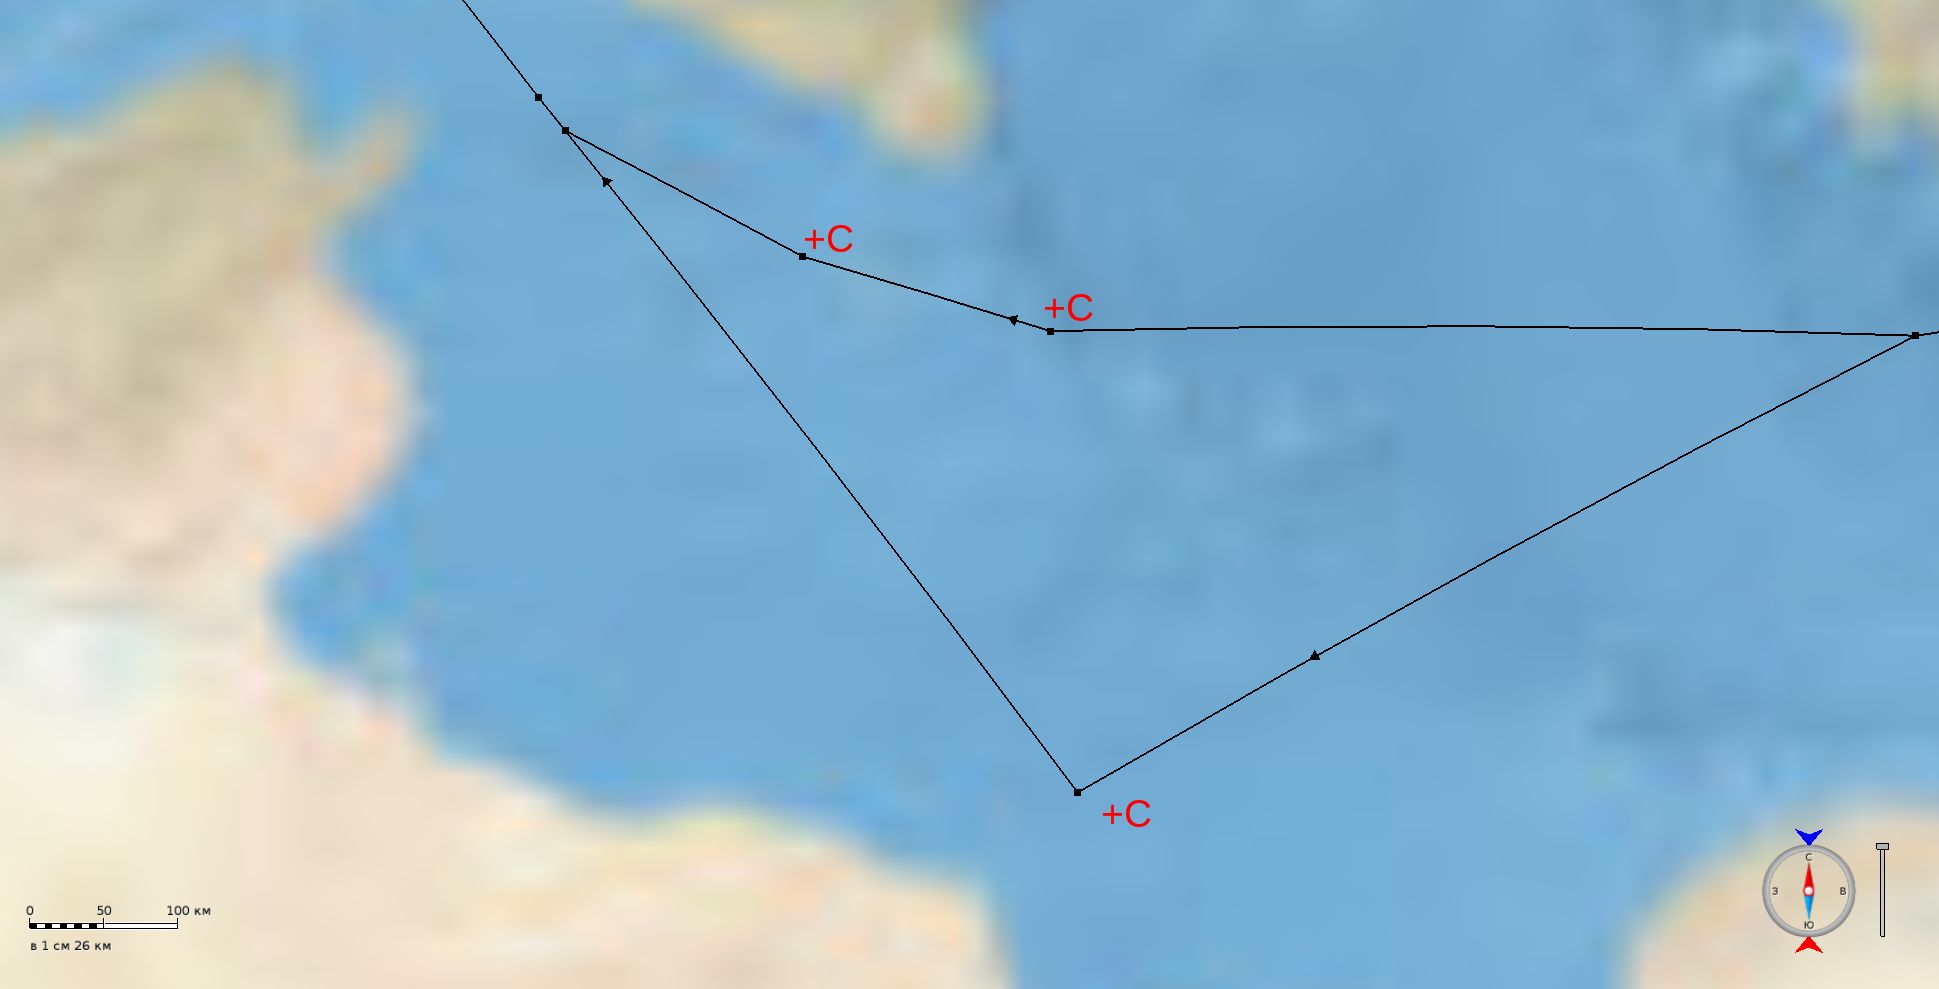
\includegraphics[width=\textwidth, clip=true, trim = 120 200 0
    0]{Solution/potentials-multipliers}
    \caption{Потенциалы должны быть множителями}
    \label{fig:potentials-multipliers}
\end{figure}

Рассмотрим рисунок~\ref{fig:potentials-multipliers}. На данном рисунке
между крайней правой и крайней левой точкой есть два альтернативных
пути. Предположим, что до этого был найдены длинные маршруты (хотя бы
один), в окрестность которых попадают изображённые вершины. В этом
случае, поскольку эти вершины находятся близко друг к другу, их
потенциалы будут примерно равны некоторому $C$. Тогда, если
использовать предложенный выше подход, то увеличение веса верхнего
пути за счёт потенциалов будет на $C$ больше, чем увеличение веса
нижнего пути. Из-за этого будет выбран более длинный нижний путь.
Таким образом, возникает проблема в том, что вес пути начинает
зависеть от числа вершин в нём. Более осмысленно использовать
потенциалы как множители, например, домножать веса рёбер на среднее
геометрическое потенциалов инцидентных вершин. В этом случае
увеличение веса подпути при примерно равных потенциалах не будет
зависеть от количества вершин. При этом значение потенциала в таком
случае должно быть безразмерной величиной, и изначально для каждой
вершины оно равно единице (что соответствует немодифицированным весам
рёбер). Поскольку потенциал должен увеличивать вес ребра, то его
значение не может быть меньше единицы. Для максимального значения
потенциала вводится отдельный параметр $max\_potential$. Как уже
отмечалось, потенциал вершины $v$ должен убывать с ростом расстояния
от фиктивной вершины до неё ($d[v]$). Поэтому для вычисления
потенциала используется эвристическая функция:
$1 + (max\_potential - 1) \cdot \frac{limit - d[v]}{limit}$. Она
удовлетворяет следующим свойствам:
\begin{itemize}
    \item Значение потенциала принадлежит отрезку $[1 .. max\_potential]$.
    \item Значение потенциала убывает с ростом расстояния от фиктивной
      вершины.
    \item Для вершин, расстояние до которых равно максимальному, значение
      потенциала минимально.
\end{itemize}

\begin{figure}
    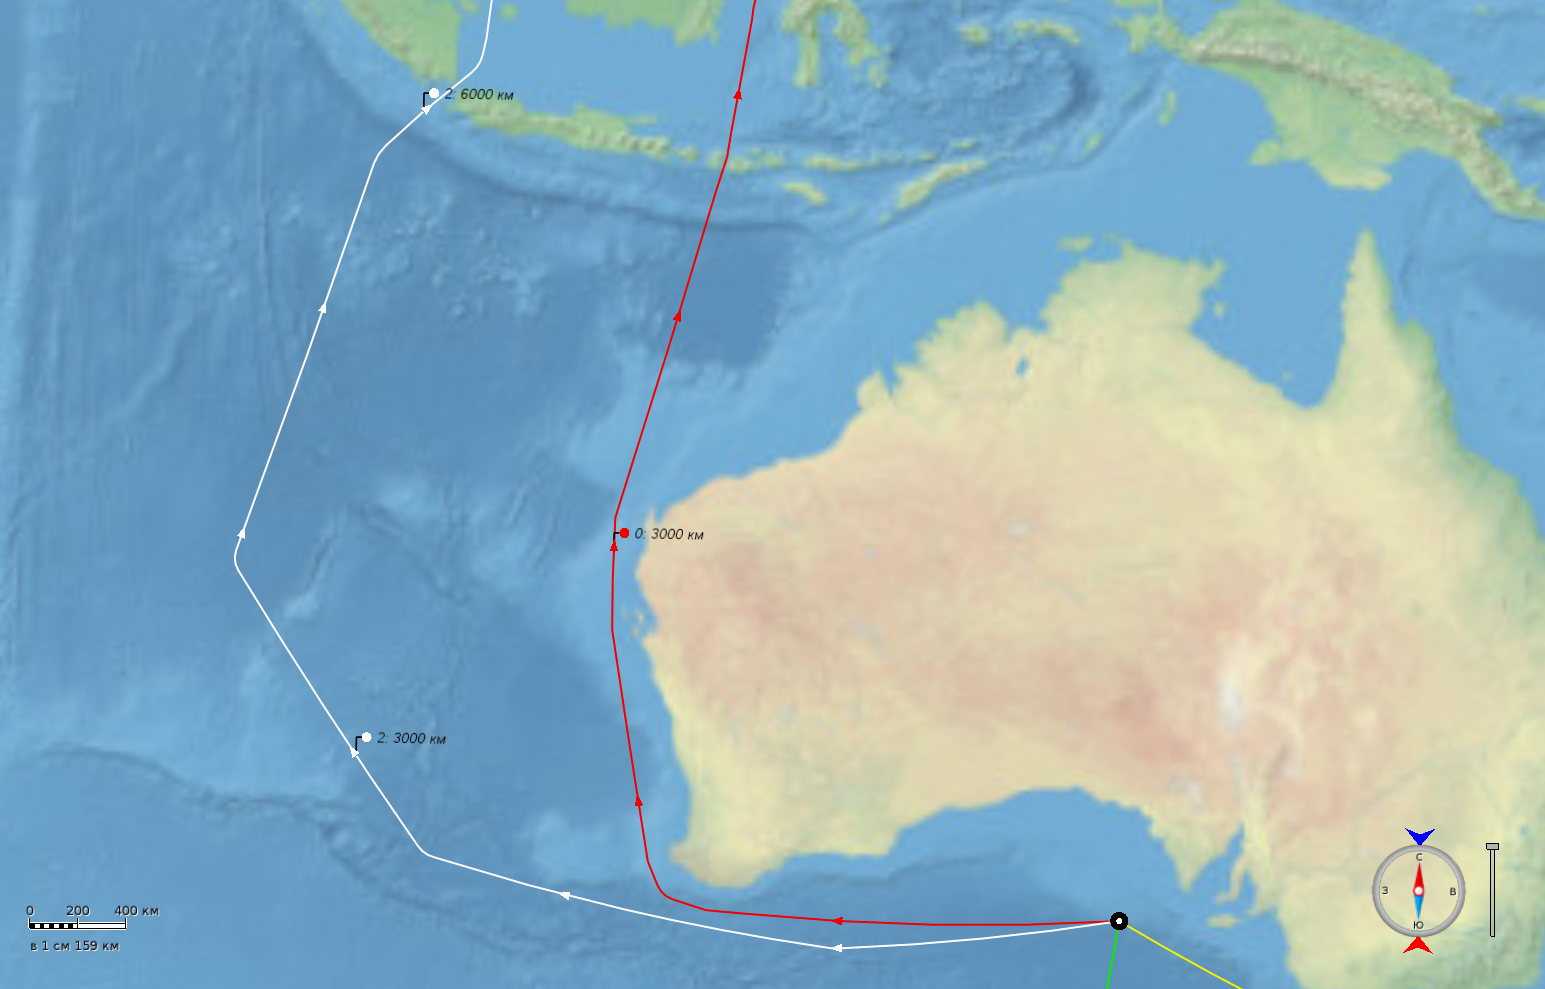
\includegraphics[width=\textwidth, clip=true, trim = 200 0 300
    0]{Solution/weights-on-path-bad}
    \caption{Маршруты несущественно разошлись}
    \label{fig:weights-on-path-bad}
\end{figure}

\begin{figure}
    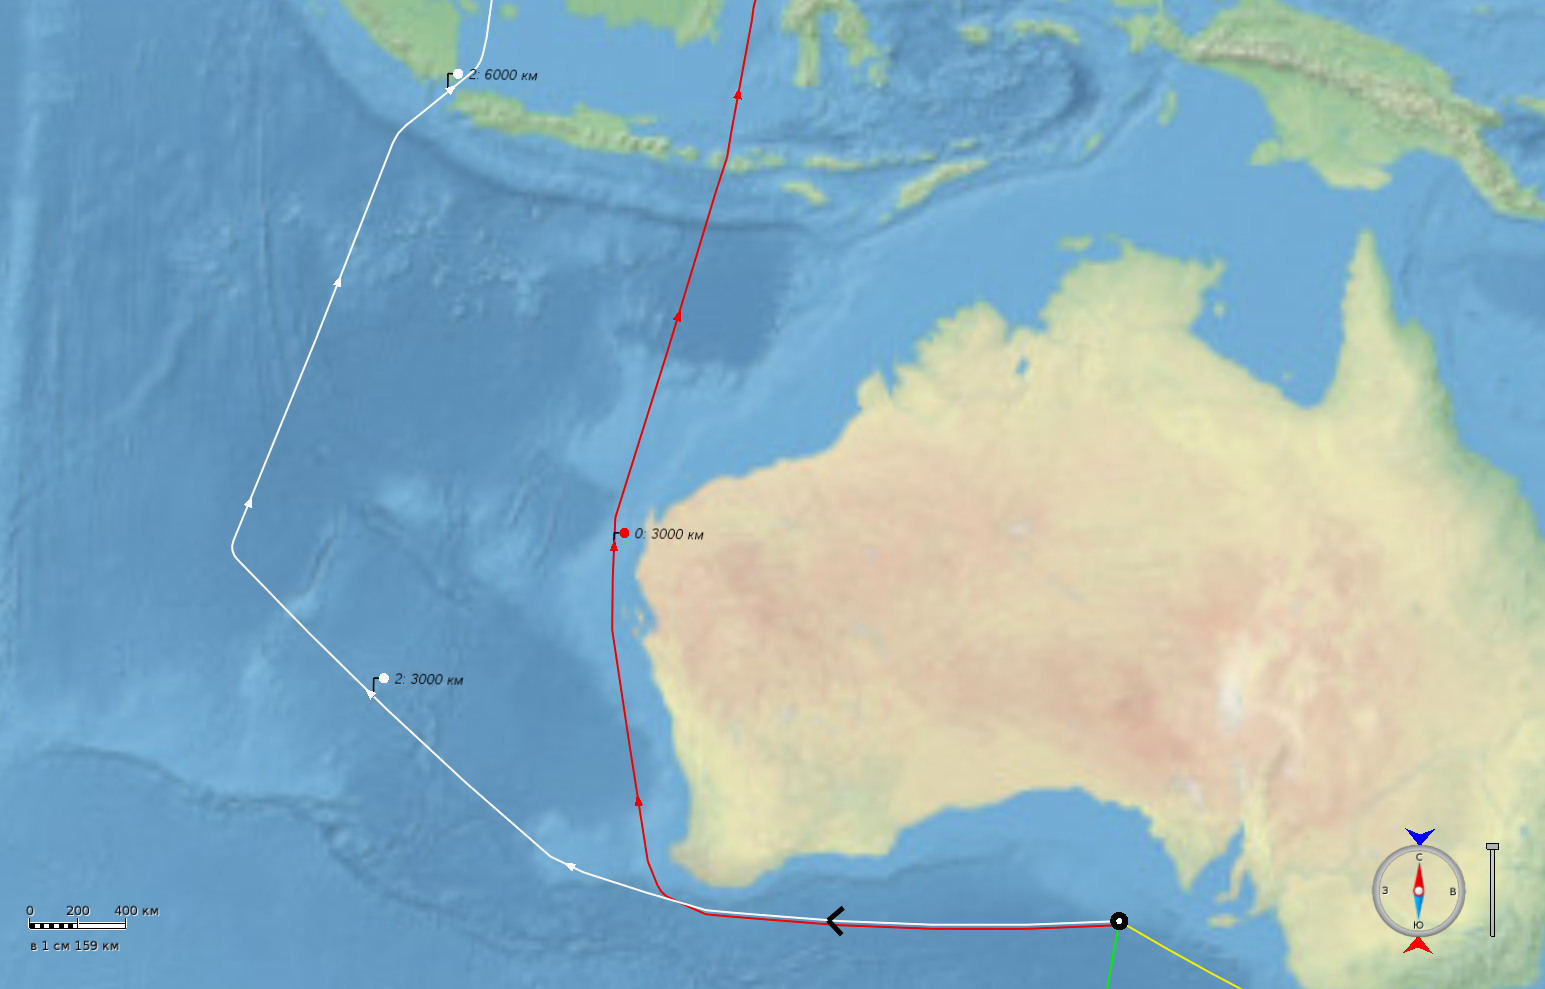
\includegraphics[width=\textwidth, clip=true, trim = 200 0 300
    0]{Solution/weights-on-path-good}
    \caption{Маршруты совпадают и оптимальны в начале}
    \label{fig:weights-on-path-good}
\end{figure}

Описанный выше способ обновления весов рёбер обладает недостатком,
проиллюстрированным на рисунке~\ref{fig:weights-on-path-bad}. Проблема
заключается в том, что для вершин найденного маршрута значение
потенциалов максимально (поскольку расстояние от фиктивной вершины
равно нулю). В связи с этим следующий найденный маршрут будет
проходить на небольшом расстоянии от предыдущего. При этом он станет
длиннее, но не станет непохожим в смысле сформулированного ранее
критерия. Разумеется, такое поведение является неестественным и не
удовлетворяет неформальной постановке задачи. Поэтому кратчайшие
расстояния от фиктивной вершины до вершин на маршруте принимаются
равными $\frac{limit}{M}$, где $M > 1$ --- параметр алгоритма. За счёт
этого в приведённом примере южная часть белого маршрута совпала с той
же частью красного, проходящего по кратчайшему пути
(рис.~\ref{fig:weights-on-path-good}).

\begin{figure}
    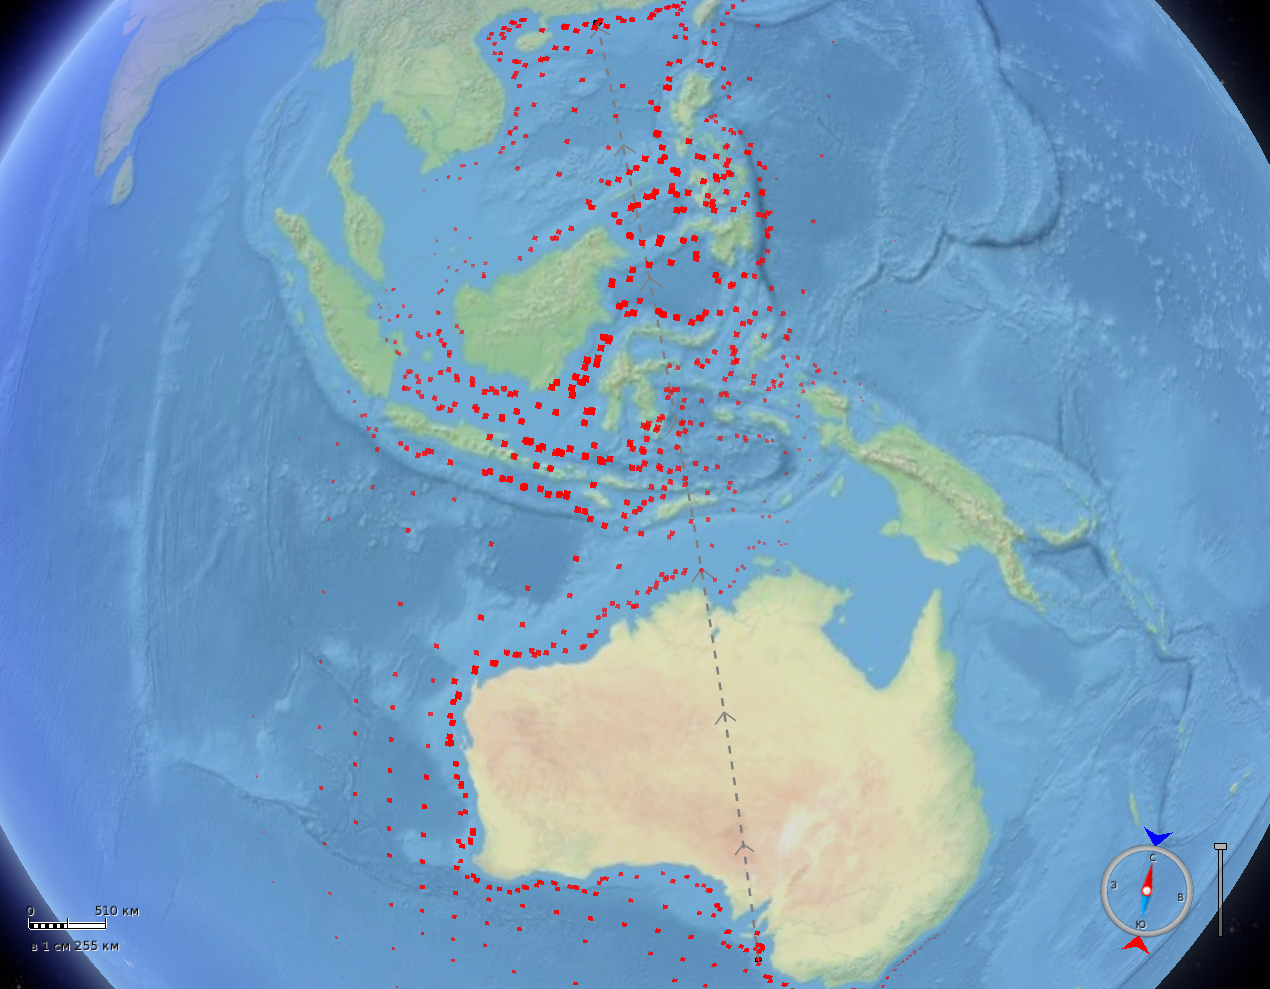
\includegraphics[width=\textwidth]{Solution/potentials-update/accum1}
    \caption{Обновление потенциалов: умножение (1)}
    \label{fig:update-accum1}
\end{figure}

\begin{figure}
    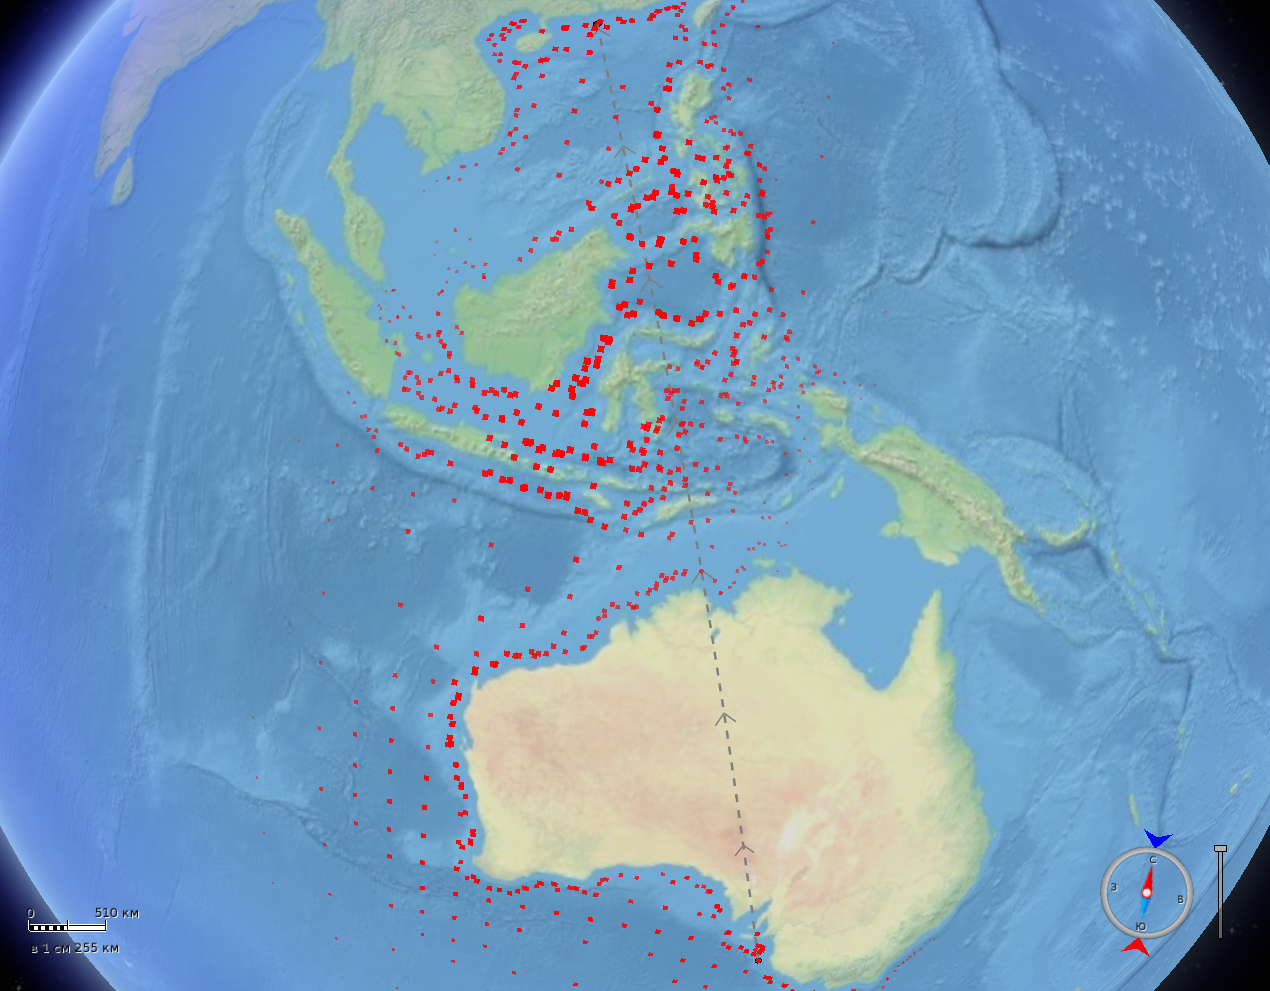
\includegraphics[width=\textwidth]{Solution/potentials-update/max1}
    \caption{Обновление потенциалов: максимум (1)}
    \label{fig:update-max1}
\end{figure}

\begin{figure}
    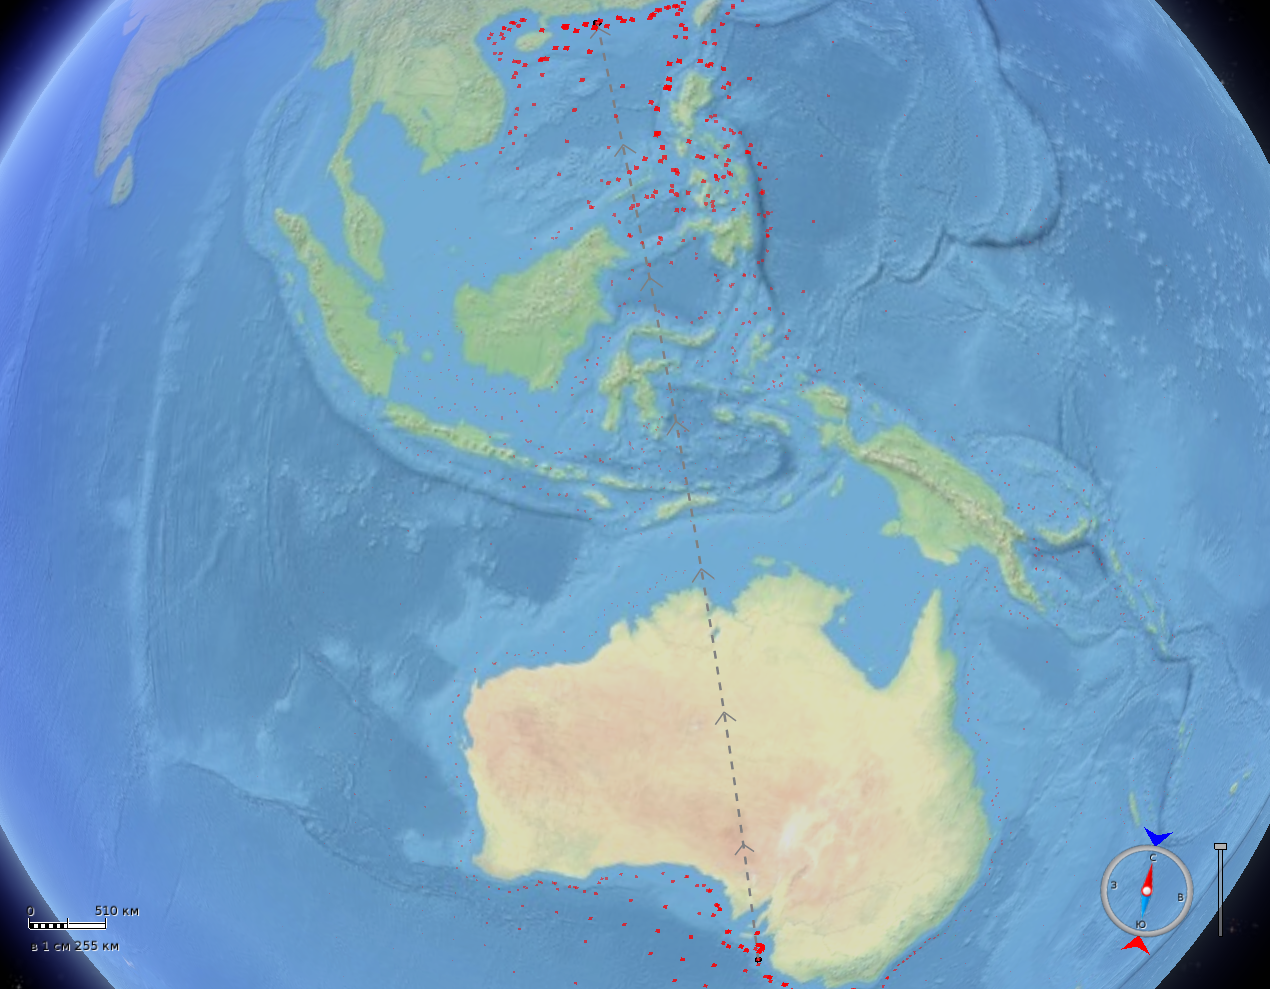
\includegraphics[width=\textwidth]{Solution/potentials-update/accum2}
    \caption{Обновление потенциалов: умножение (2)}
    \label{fig:update-accum2}
\end{figure}

\begin{figure}
    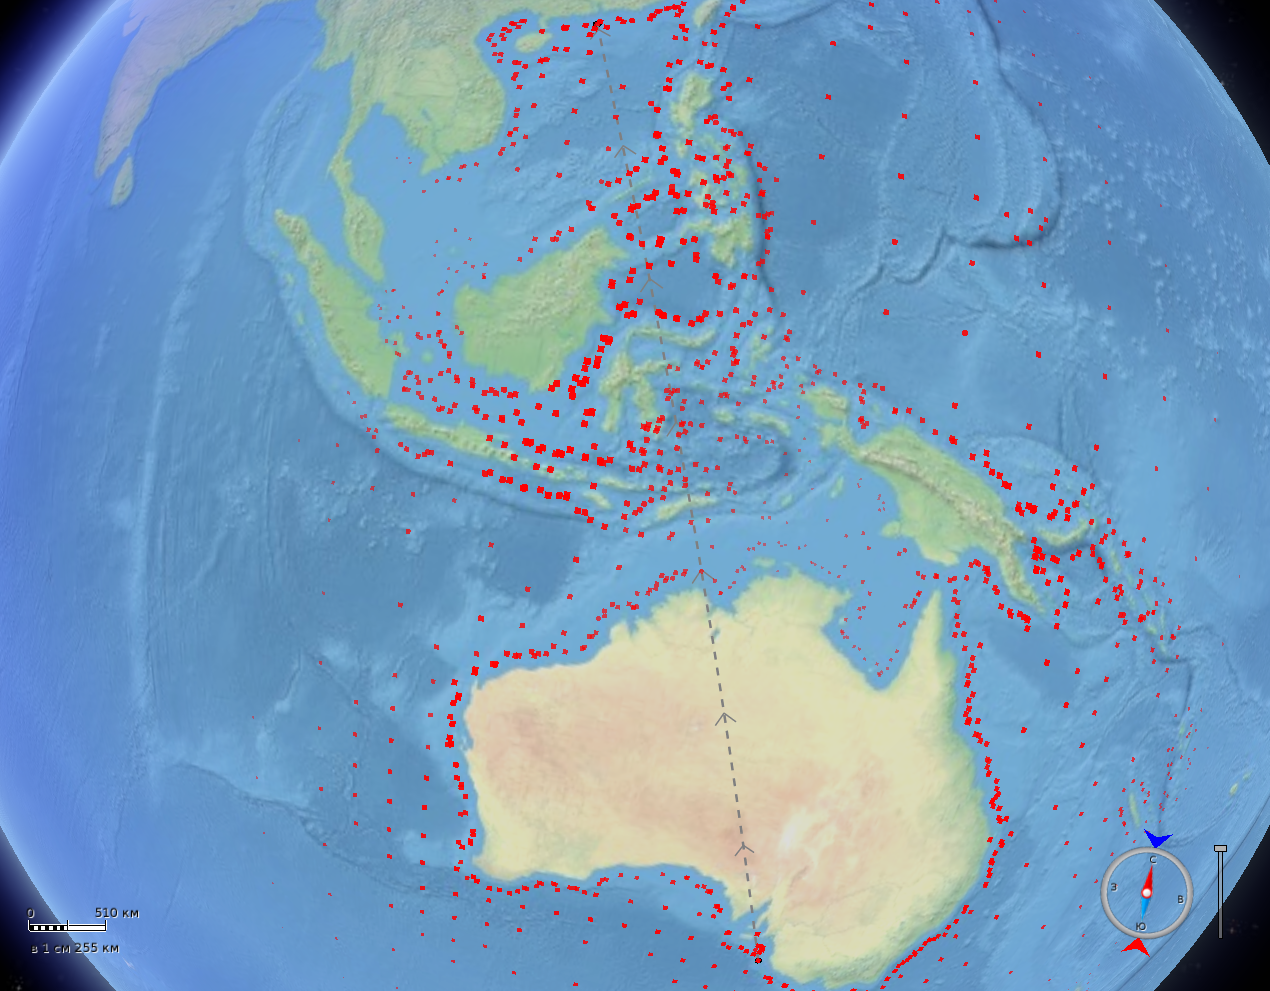
\includegraphics[width=\textwidth]{Solution/potentials-update/max2}
    \caption{Обновление потенциалов: максимум (2)}
    \label{fig:update-max2}
\end{figure}

\begin{figure}
    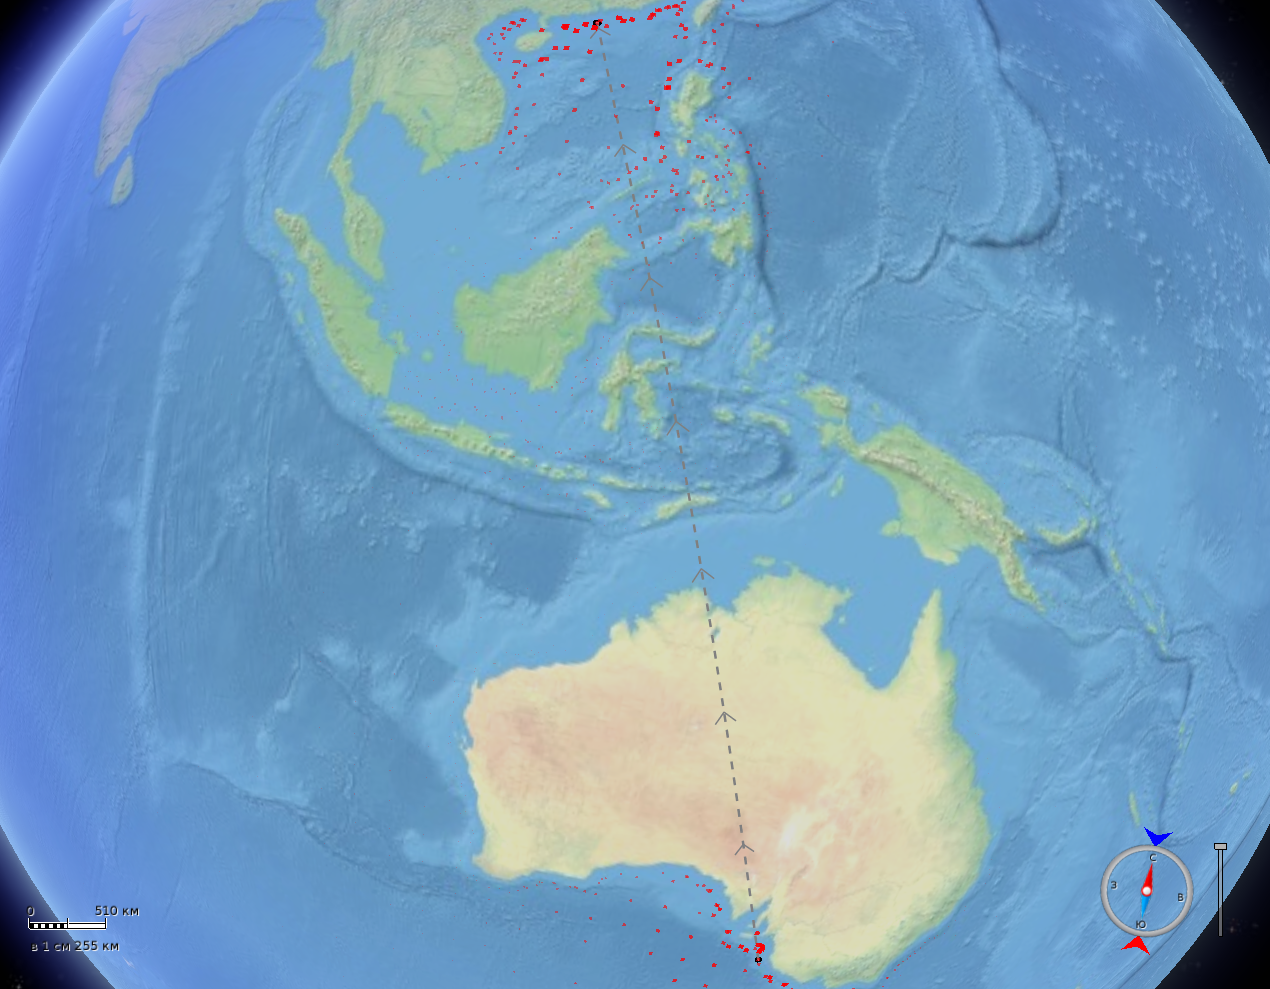
\includegraphics[width=\textwidth]{Solution/potentials-update/accum3}
    \caption{Обновление потенциалов: умножение (3)}
    \label{fig:update-accum3}
\end{figure}

\begin{figure}
    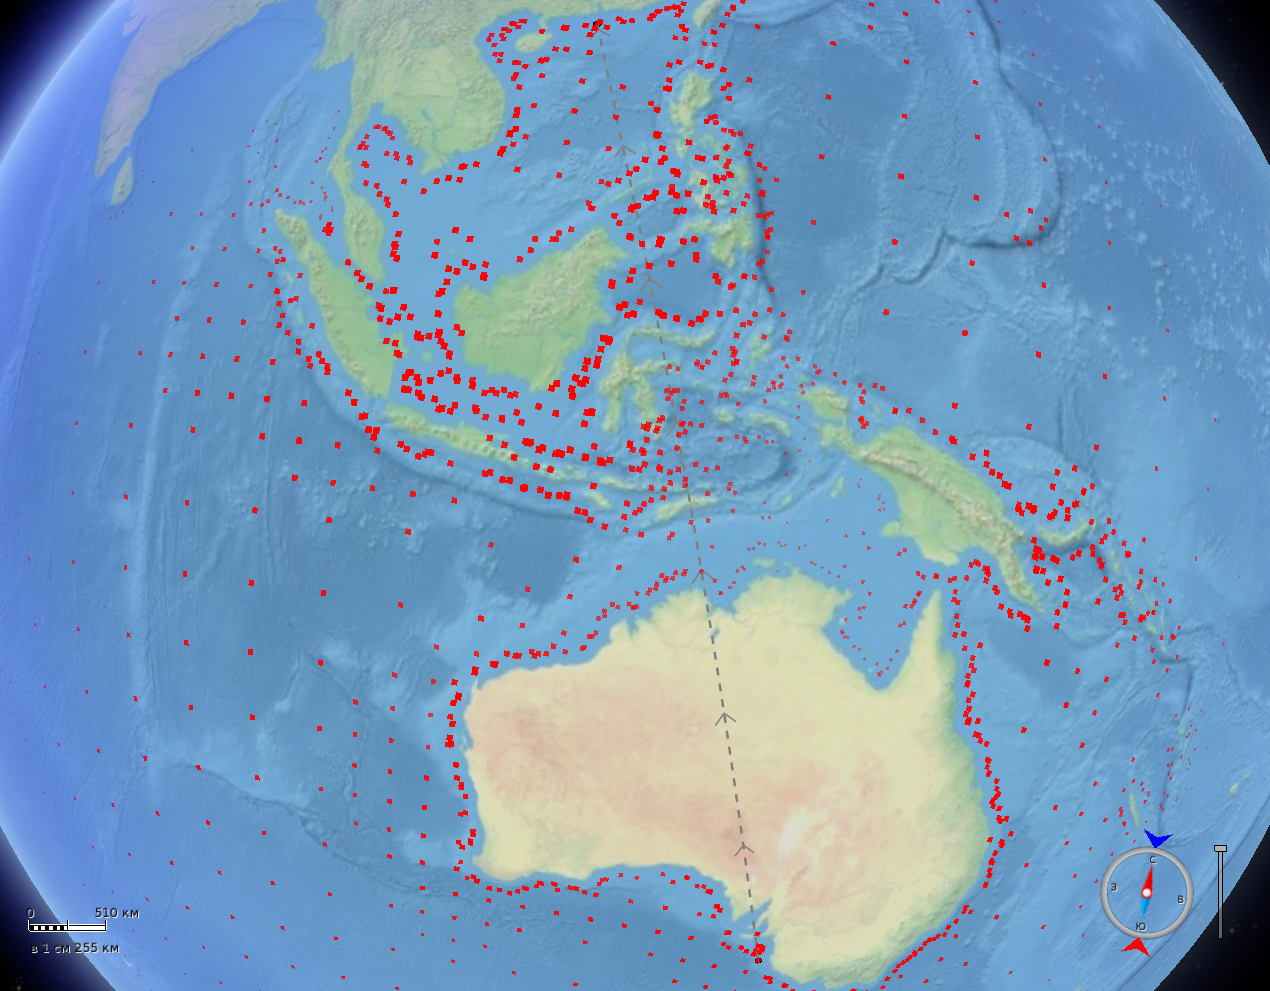
\includegraphics[width=\textwidth]{Solution/potentials-update/max3}
    \caption{Обновление потенциалов: максимум (3)}
    \label{fig:update-max3}
\end{figure}

\begin{figure}
    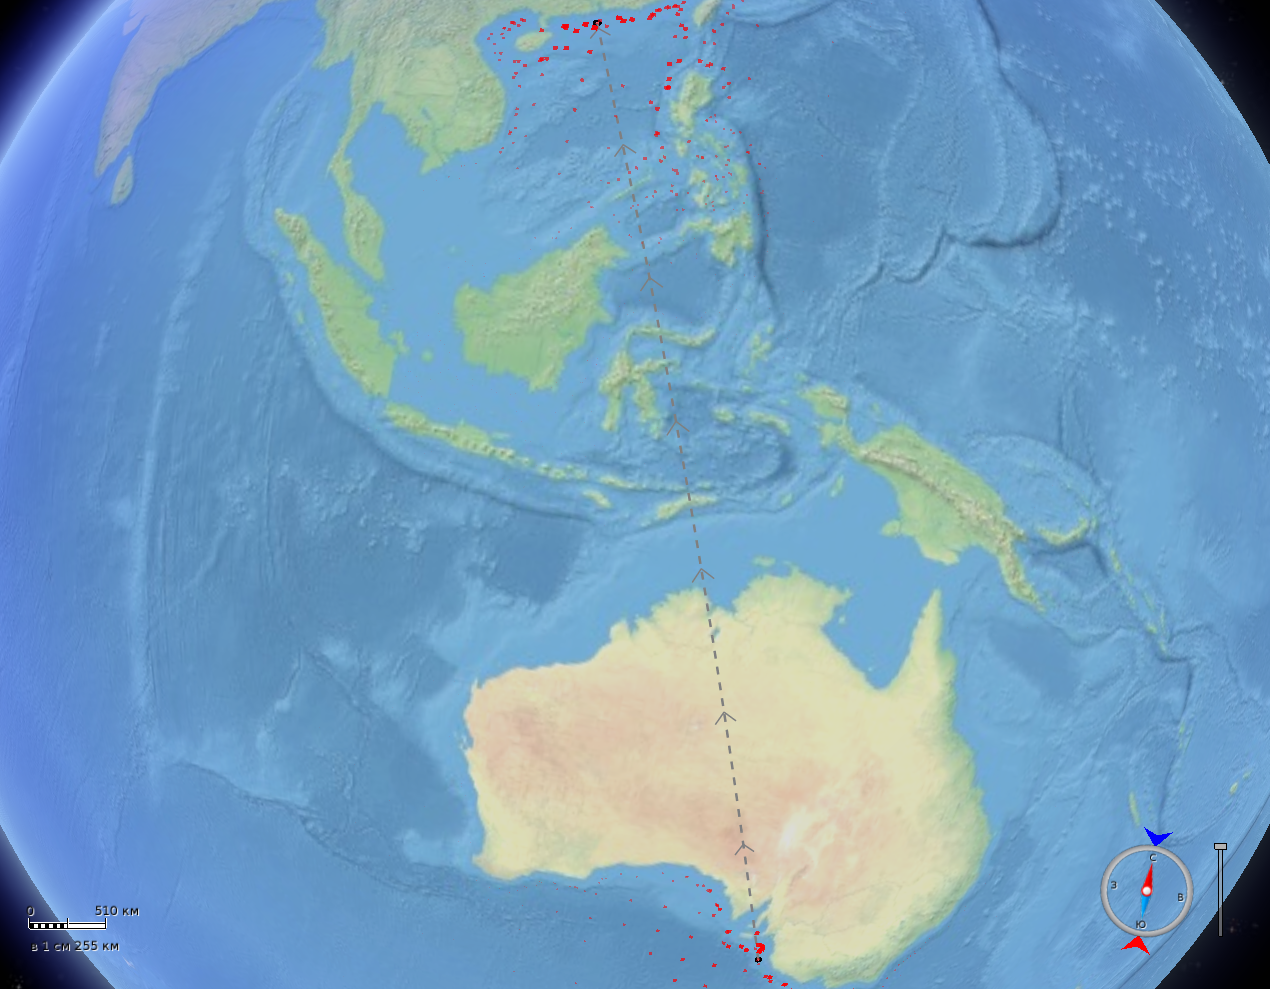
\includegraphics[width=\textwidth]{Solution/potentials-update/accum4}
    \caption{Обновление потенциалов: умножение (4)}
    \label{fig:update-accum4}
\end{figure}

\begin{figure}
    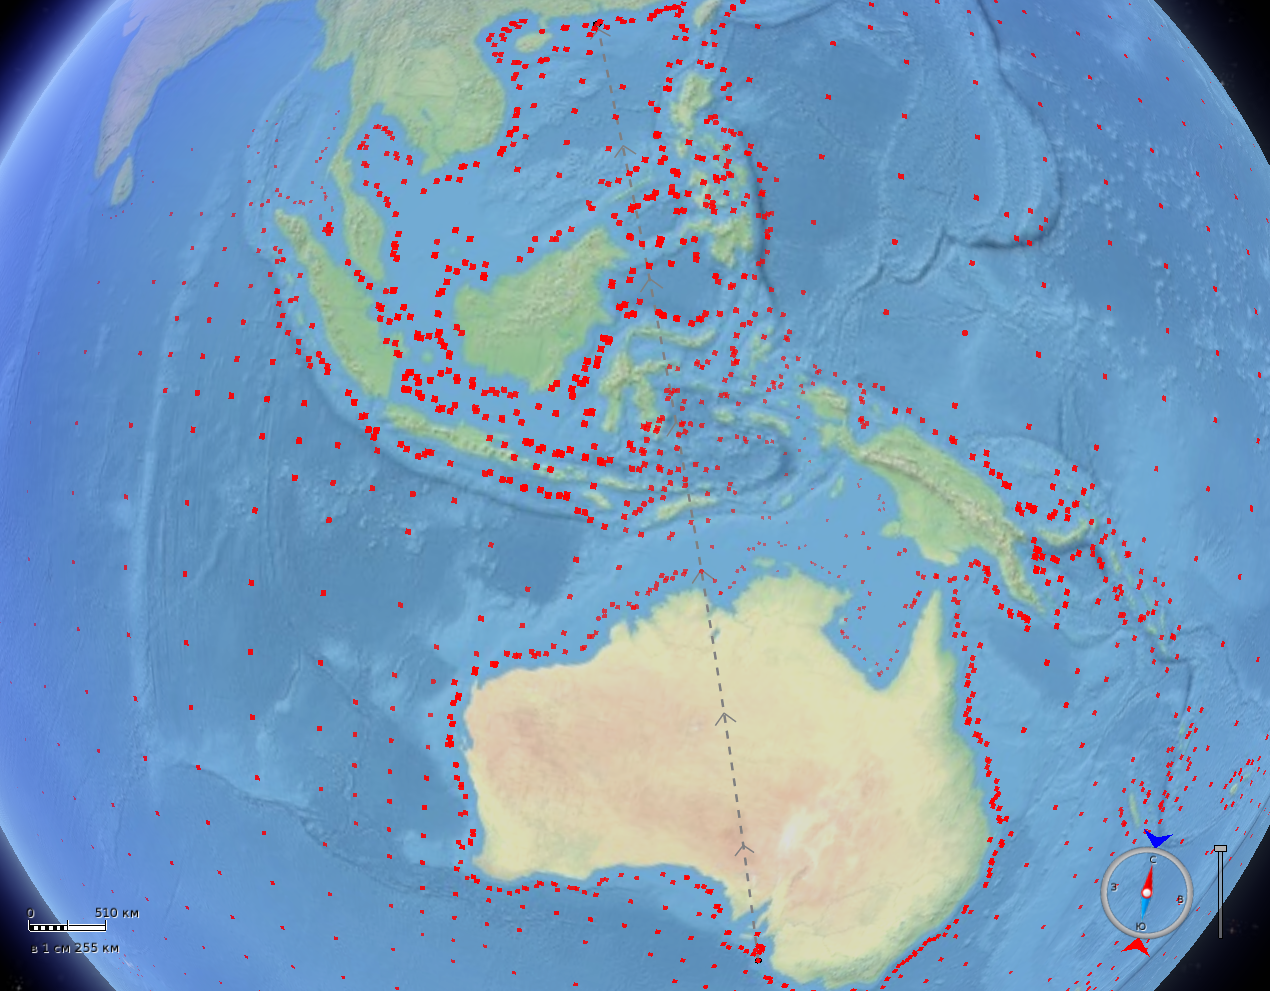
\includegraphics[width=\textwidth]{Solution/potentials-update/max4}
    \caption{Обновление потенциалов: максимум (4)}
    \label{fig:update-max4}
\end{figure}

\begin{figure}
    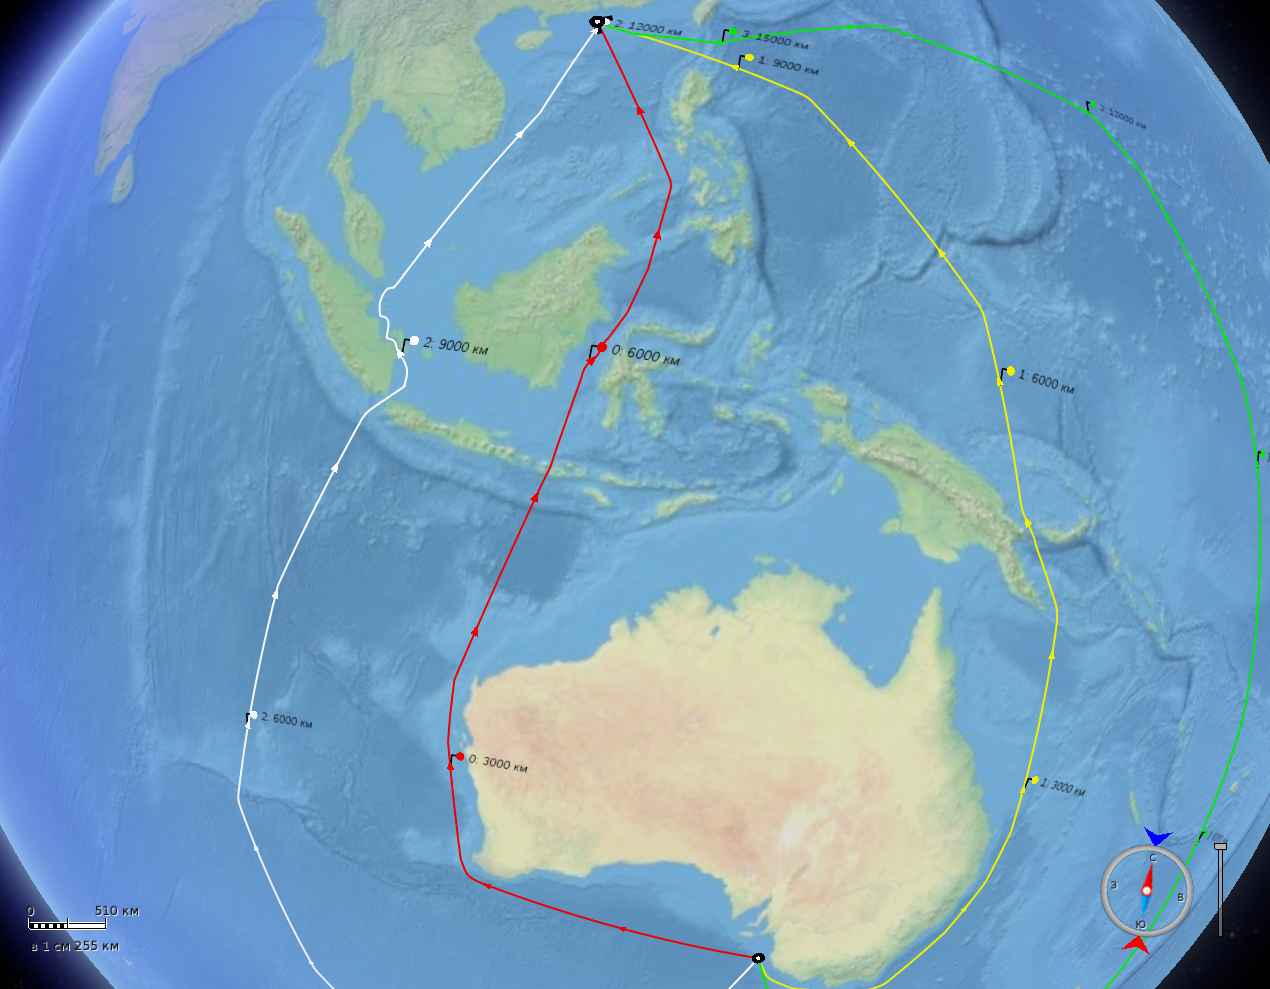
\includegraphics[width=\textwidth]{Solution/potentials-update/accum_result}
    \caption{Найденные маршруты при использовании умножения}
    \label{fig:update-accum-result}
\end{figure}

\begin{figure}
    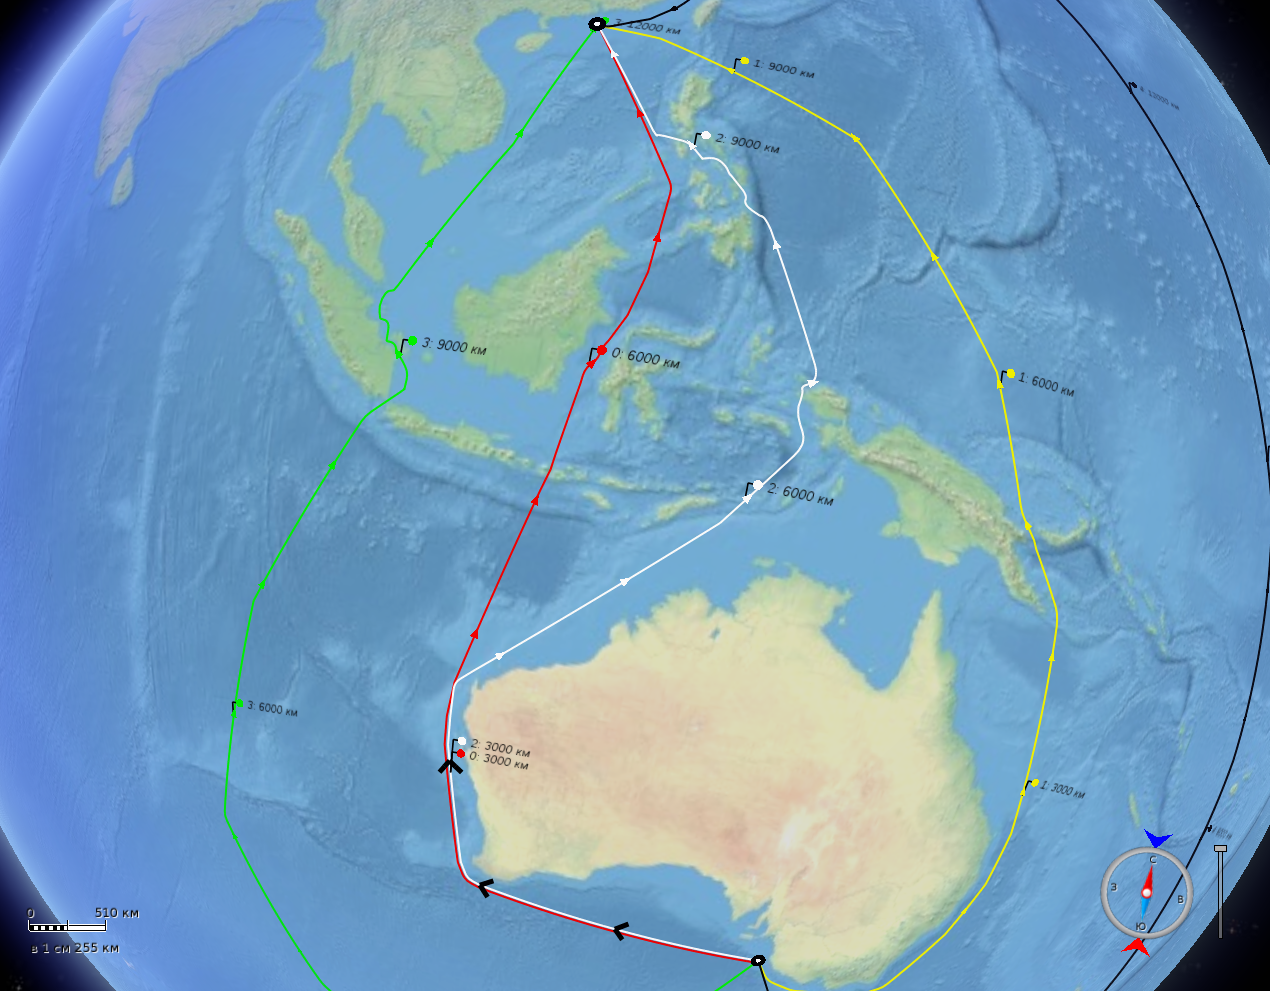
\includegraphics[width=\textwidth]{Solution/potentials-update/max_result}
    \caption{Найденные маршруты при использовании максимума}
    \label{fig:update-max-result}
\end{figure}

Наконец, последний вопрос состоит в обновлении потенциалов, после того
как найден очередной маршрут. Понятно, что потенциалы должны как-то
накапливаться, чтобы учитывать влияние всех предыдущих маршрутов и не
допускать прохождение нового маршрута вблизи старых. Например, можно
для каждой вершины в качестве нового потенциала брать сумму или
произведение имеющегося потенциала и вновь посчитанного. Также можно
брать максимум. На
рисунках~(\ref{fig:update-accum1}--\ref{fig:update-max4})
проиллюстрированы различия между двумя вариантами: перемножением и
максимумом. Красные квадраты визуализируют значения потенциалов: чем
больше и ярче квадрат, тем больше потенциал. После нахождения первого
маршрута потенциалы, очевидно, распределены одинаково
(рис.~\ref{fig:update-accum1} и \ref{fig:update-max1}). Затем, если
перемножать потенциалы, то для вершин в окрестностях начальной и
конечной точек они оказываются сильно больше, чем для остальных
вершин~(рис.~\ref{fig:update-accum2}). Если же брать максимум, то
распространение потенциалов происходит равномерно: во всех точках,
расположенных близко к какому-либо найденному маршруту, потенциал
оказывается большой~(\ref{fig:update-max2}).
Рисунки~(\ref{fig:update-accum3}--\ref{fig:update-max4})
демонстрируют, что в дальнейшим описанный эффект лишь усиливается. В
результате проведённого эксперимента при использовании максимума для
обновления потенциалов было найдено на один маршрут
больше~(рис.~\ref{fig:update-accum-result}--\ref{fig:update-max-result}).
Поэтому в предложенном алгоритме используется максимум для обновления
потенциалов.

\FloatBarrier


%-*-coding: utf-8-*-
\chapter{Практическая реализация и результаты}

\label{ch:implementation}

В данной главе рассмотрены некоторые аспекты практической реализации
предложенного алгоритма и визуализации. Программный модуль, решающий
поставленную задачу, был реализован на языке C++ в рамках имеющегося
фреймворка для решения задач. В заключение приводятся основные
результаты работы.

\FloatBarrier

\section{Предобработка}

\label{sec:preprocessing-impl}

Для решения большей части задач по предобработке данных использованы
библиотеки ЗАО «Кронштадт Технологии». Чтение исходных данных и
классификация объектов карты осуществляется с помощью имеющихся утилит
импорта картографических данных. Для выполнения геометрических
операций, таких как объединение контуров, упрощение полилиний,
построение straight skeleton, смещение полигона и т. д., используется
библиотека геометрических примитивов и алгоритмов ЗАО «Кронштадт
Технологии». Также в этой библиотеке есть специальная структура
данных, названная \emph{Contours Set}, для эффективной проверки
пересечения отрезка с полигоном. Эта структура данных активно
используется для всех проверок корректности рёбер (при добавлении
рёбер, сглаживании маршрута, упрощении цепочек рёбер straight
skeleton'а).

\begin{figure}
    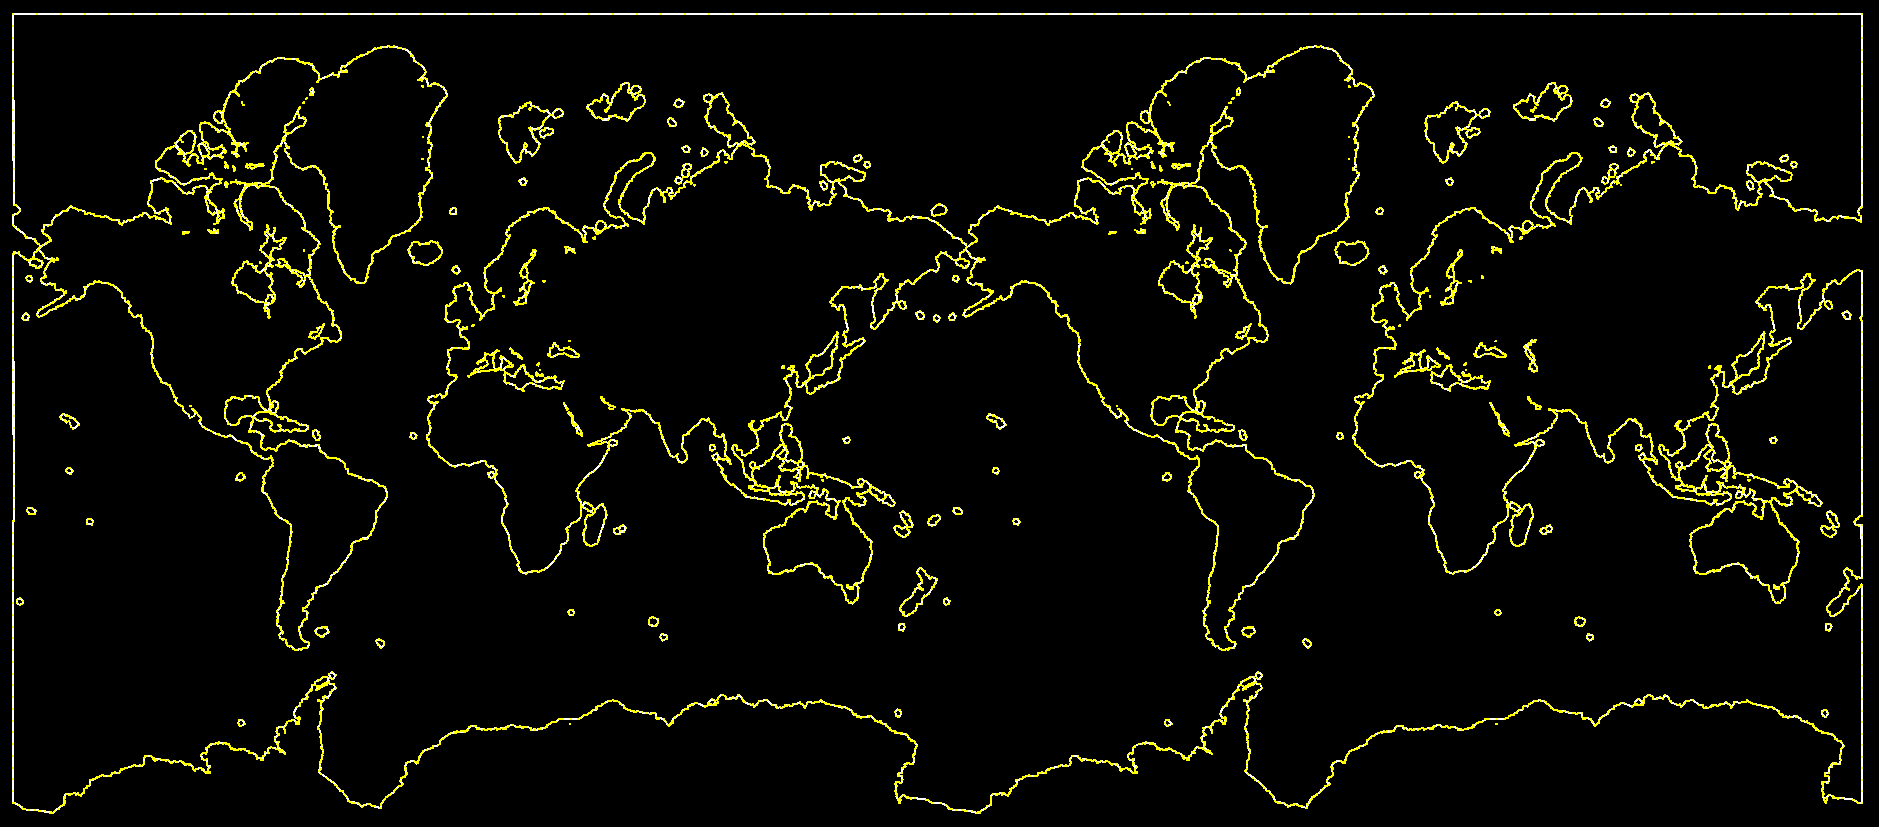
\includegraphics[width=\textwidth]{Solution/doubled-offseted-polygon}
    \caption{Полигон, объединённый со смещённой копией}
    \label{fig:doubled-polygon}
\end{figure}

Определённую сложность представляет добавление рёбер через 180-ый
меридиан. Для этого имеющийся полигон, ограничивающий воду,
объединяется со своей копией, сдвинутой влево на длину плоскости
проекции. В результате получается полигон, изображённый на
рисунке~\ref{fig:doubled-polygon}. По такому полигону можно легко
проверять корректность ребра, проходящего через 180-ый меридиан,
переместив его восточную точку влево на длину плоскости проекции.

Для тестирования работы алгоритма использовались свободно
распространняемые данные OpenStreetMap~\cite{osm}. Получившийся граф
содержит 13344 вершины и 124324 ребра.

\FloatBarrier

\section{Вычисление метрик}

\label{sec:metrics-computation}

Поскольку в процессе работы алгоритма для всех пар путей проверяется
критерий похожести, необходимо добиться высокой скорости вычисления
метрик на маршрутах. Для вычисления обеих метрик используются длины
кратчайших расстояний между парами вершин в графе. Длины кратчайших
расстояний между всеми парами вершин могут быть найдены с помощью
алгоритма Флойда~\cite{floyd1962algorithm}. Однако алгоритм Флойда
работает за время порядка $\Theta(n^3)$, что неприемлимо для графа,
содержащего 13344 вершины. Также нетрудно заметить, что знать длины
кратчайших путей в графе между всеми парами вершин не нужно, поскольку
в определении обеих метрик присутствуют лишь длины кратчайших путей
для всех пар вершин, принадлежащих первому и второму маршруту. Поэтому
можно для каждой вершины первого пути использовать алгоритм Дейкстры и
останавливать поиск при достижении какой-либо вершины второго пути.
Поскольку в этом случае время работы сильно зависит от конкретных
маршрутов (не только от числа вершин, но и от их расположения,
поскольку каждый поиск алгоритмом Дейкстры может заканчиваться очень
рано или, наоборот, спустя большое число итераций), то теоретические
оценки времени работы такого подхода не несут практической информации.
На практике же при таком способе вычисления метрик поиск маршрутов,
как правило, занимал 2--10 секунд. Однако поставленная задача требует
выполнять запросы за время, не превышающее одной секунды.

Для улучшения производительности было сделано две оптимизации.
Нетрудно заметить, что если в процессе вычисления первой метрики
находится пара вершин из первого и второго маршрута, между которыми
длина кратчайшего пути в графе больше порогового значения, то можно
заключить, что маршруты непохожи. При вычислении второй метрики верен
аналогичный факт. Таким образом, поскольку метрики считаются только
для проверки критерия похожести маршрутов, то вычисление можно
останавливать, как только найдена пара вершин, гарантирующая
непохожесть маршрутов.

Вторая оптимизация затрагивает сам процесс вычисления метрик. Вместо
поиска кратчайших расстояний с помощью алгоритма Дейкстры из всех
вершин пути используется другой подход. Сначала строится граф с
фиктивной вершиной~($f$), из которой проведены рёбра нулевого веса во
все вершины первого маршрута~($P$). Затем с помощью алгоритма Дейкстры
находятся длины кратчайших расстояний из фиктивной вершины до всех
вершин второго маршрута~($Q$) (поиск заканчивается, когда посещены все
вершины, принадлежащие $Q$). Поскольку из фиктивной вершины проведены
рёбра нулевого веса во все вершины, принадлежащие $P$, и только в них,
то кратчайший путь от неё до вершины $v \in Q$ будет иметь вид
$fu \dots v$ для какой-то вершины $u \in P$, и его длина будет равна
$\rho_g(u, v)$. Как и в определении метрик за $\rho_g(u, v)$
обозначена длина кратчайшего пути между вершинами $u$ и $v$ в графе.
Нетрудно заметить, что в этом случае
$\rho_g(u, v) = \min\limits_{w \in P} \rho_g(w, v)$. Действительно,
пусть существует вершина $u' \in P$, такая что
$\rho_g(u', v) < \rho_g(u, v)$. Обозначим кратчайший путь в графе
между $u'$ и $v$ как $R = u'r_0r_1 \dots r_nv$. Тогда длина пути
$fu'r_0 \dots r_nv$ равна
$\rho_g(u', v) < \rho_g(u, v) = \rho_g(f, v)$, что противоречит тому,
что $\rho_g(f, v)$ является длиной кратчайшего пути из $f$ в $v$.
Значит, предположение о существовании $u'$ неверно. Таким образом,
сразу для всех вершин $v \in Q$ находится величина
$\min\limits_{u \in P} \rho_(u, v)$ за один обход алгоритма Дейкстры.
Аналогичный поиск можно выполнить, добавив фиктивную вершину и рёбра
нулевого веса во все вершины маршрута $Q$, тем самым найдя для всех
$u \in P$ величину $\min\limits_{v \in Q} \rho_(u, v)$. После этого
достаточно взять максимум всех найденных величин, который будет
значением метрики. При этом, как было сказано ранее, если хоть одно из
найденных значений больше определённого порога (описанного в критерии
похожести), то вычисление можно сразу же закончить, заключив, что
маршруты непохожи. Для вычисления второй метрики помимо максимального
минимального расстояния между парами вершин нужно находить расстояние
до ближайшей вершины в мире. Данный поиск был реализован простым
перебором, работающим в худшем случае за время порядка
$\Theta(l1 \cdot l2)$, где $l1$ и $l2$ --- длины первого и второго
маршрута соответственно. Однако, во-первых, вторая метрика
вычисляется, как правило, реже, чем первая, во-вторых, зачастую не
нужно просматривать все вершины, поскольку пара вершин, для которых
выполнен критерий непохожести, встречается раньше. Помимо этого при
вычислении второй метрики не рассматриваются пары вершин, ребро между
которыми не пересекает ни одно препятствие, поскольку между такими
вершинами можно пройти по прямой. В результате проведённых оптимизаций
время обработки запроса существенно уменьшилось и стало составлять
порядка 0,2--0,8 секунды. При этом профилирование показало, что
основную часть времени стало занимать не вычисление метрик, а
сокращение маршрутов. Поскольку итоговое время работы удовлетворяет
поставленным требованиям, дальнейшие оптимизации не проводились.

\FloatBarrier

\section{Визуализация}

\label{sec:visualization-impl}

Для визуализации маршрутов была использована библиотека, разработанная в
ЗАО~«Кронштадт Технологии» и основанная на OpenGL~\cite{opengl}. Данная
библиотека позволяет отображать различные примитивы на плоскости и
сфере, в том числе полилинии на сфере. Основная проблема при
визуализации семейств маршрутов состоит в том, что некоторые маршруты
накладываются друг на друга. Решение такой проблемы состоит в смещении
перекрывающихся частей на небольшое расстояние в пикселях. Для этого
выделяются перекрывающиеся части имеющихся маршрутов (имеющие
одинаковые рёбра) с помощью сохранения рёбер в хеш-таблицу. При
визуализации каждое ребро маршрута рассматривается отдельно. Если оно
принадлежит более чем одному маршруту, то берётся порядковый номер
текущего пути в отсортированном списке маршрутов, содержащих данное
ребро, и вычисляется величина смещения путём домножения этого номера
на текущий размер пикселя в мире. Затем каждая вершина ребра смещается
на эту величину в направлении бисектрисы, проведённой в треугольнике,
образованном текущей вершиной и её соседними вершинами. Если одной из
соседних вершин не существует (вершина является начальной или конечной
точкой), то в качестве направления берётся нормаль к соответствующему
ребру. В следующем разделе приведены рисунки с примерами работы
алгоритма, на которых можно видеть смещённые маршруты.

\FloatBarrier

\section{Результаты}

\label{sec:results}

По итогам данной работы получены следующие результаты:
\begin{itemize}
    \item Исследованы имеющиеся подходы к решению аналогичных задач,
      выявлены и продемонстрированы их недостатки.
    \item Сформулировано формальное описание поставленной задачи.
    \item Предложены алгоритмы и эвристики для решения поставленной
      задачи.
    \item Реализован программный модуль, решающий поставленную задачу.
    \item Получено заключение экспертов ЗАО~«ОСК-Транзас» о том, что
      находимые маршруты удовлетворяют поставленным требованиям.
      Эвристики, разработанные для поиска различных маршрутов,
      признаны эффективными и разумными. Алгоритм и критерии,
      заложенные в программный модуль, рекомендованы для решения задач
      поддержки принятия решения в навигационно-тактических системах
      морского назначения.
    \item Разработанный программный модуль внедрён в имеющийся
      3D-клиент ЗАО~«Кронштадт Технологии».
\end{itemize}

\begin{figure}
    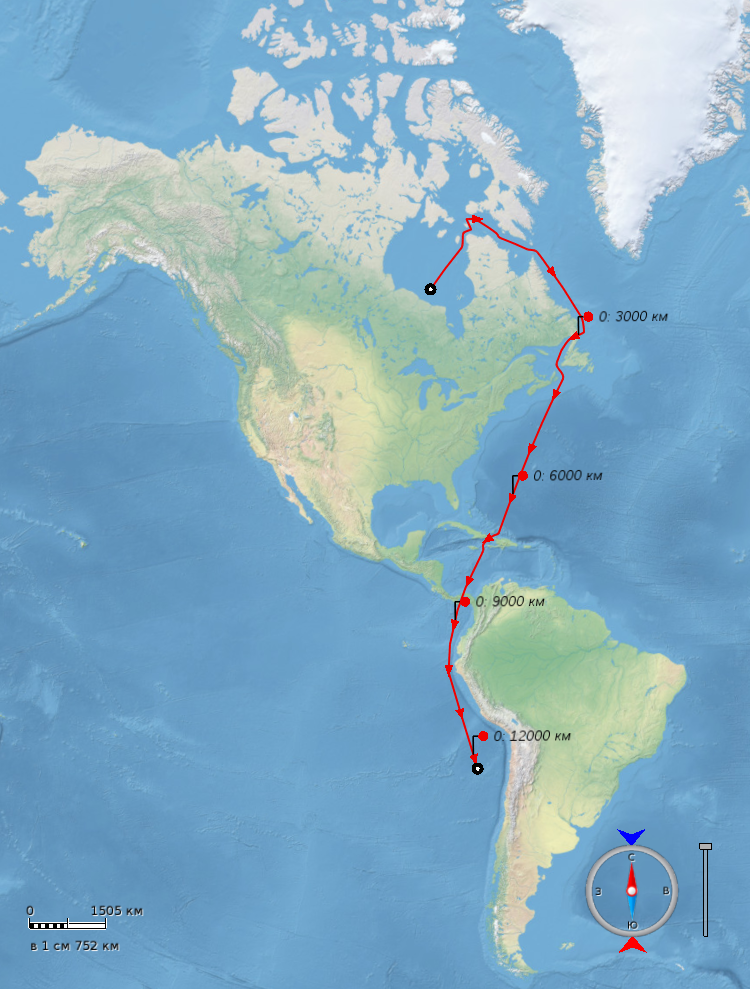
\includegraphics[width=\textwidth]{Results/comparison/bad1}
    \caption{Найден лишь один маршрут}
    \label{fig:res-comp-bad1}
\end{figure}

\begin{figure}
    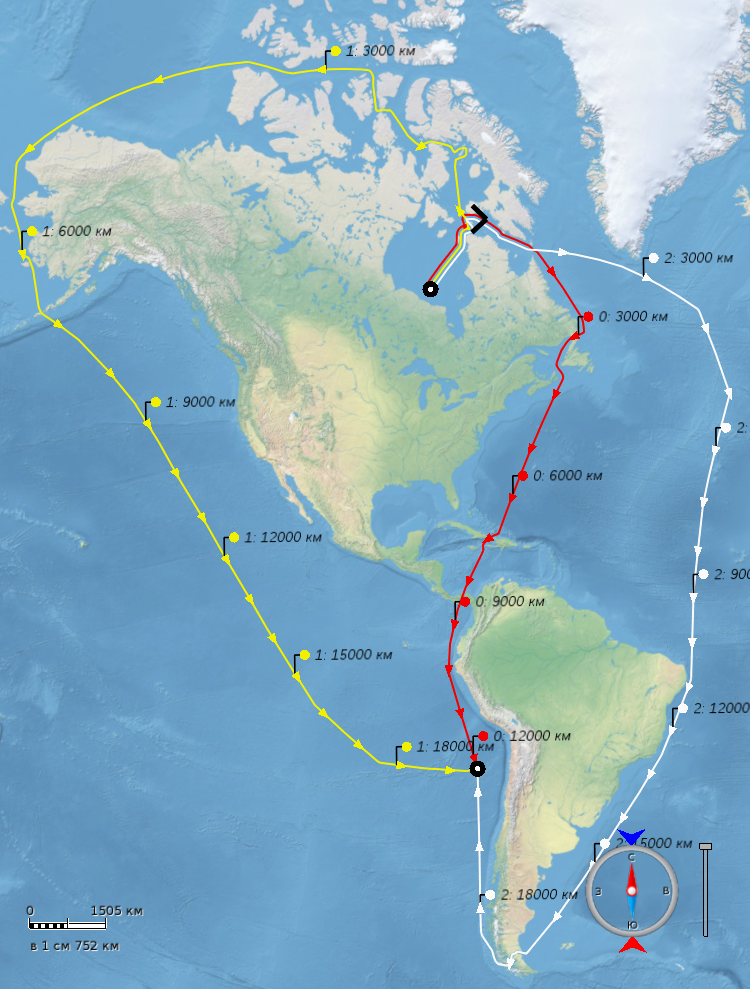
\includegraphics[width=\textwidth]{Results/comparison/good1}
    \caption{Найдено три различных маршрута}
    \label{fig:res-comp-good1}
\end{figure}

\begin{figure}
    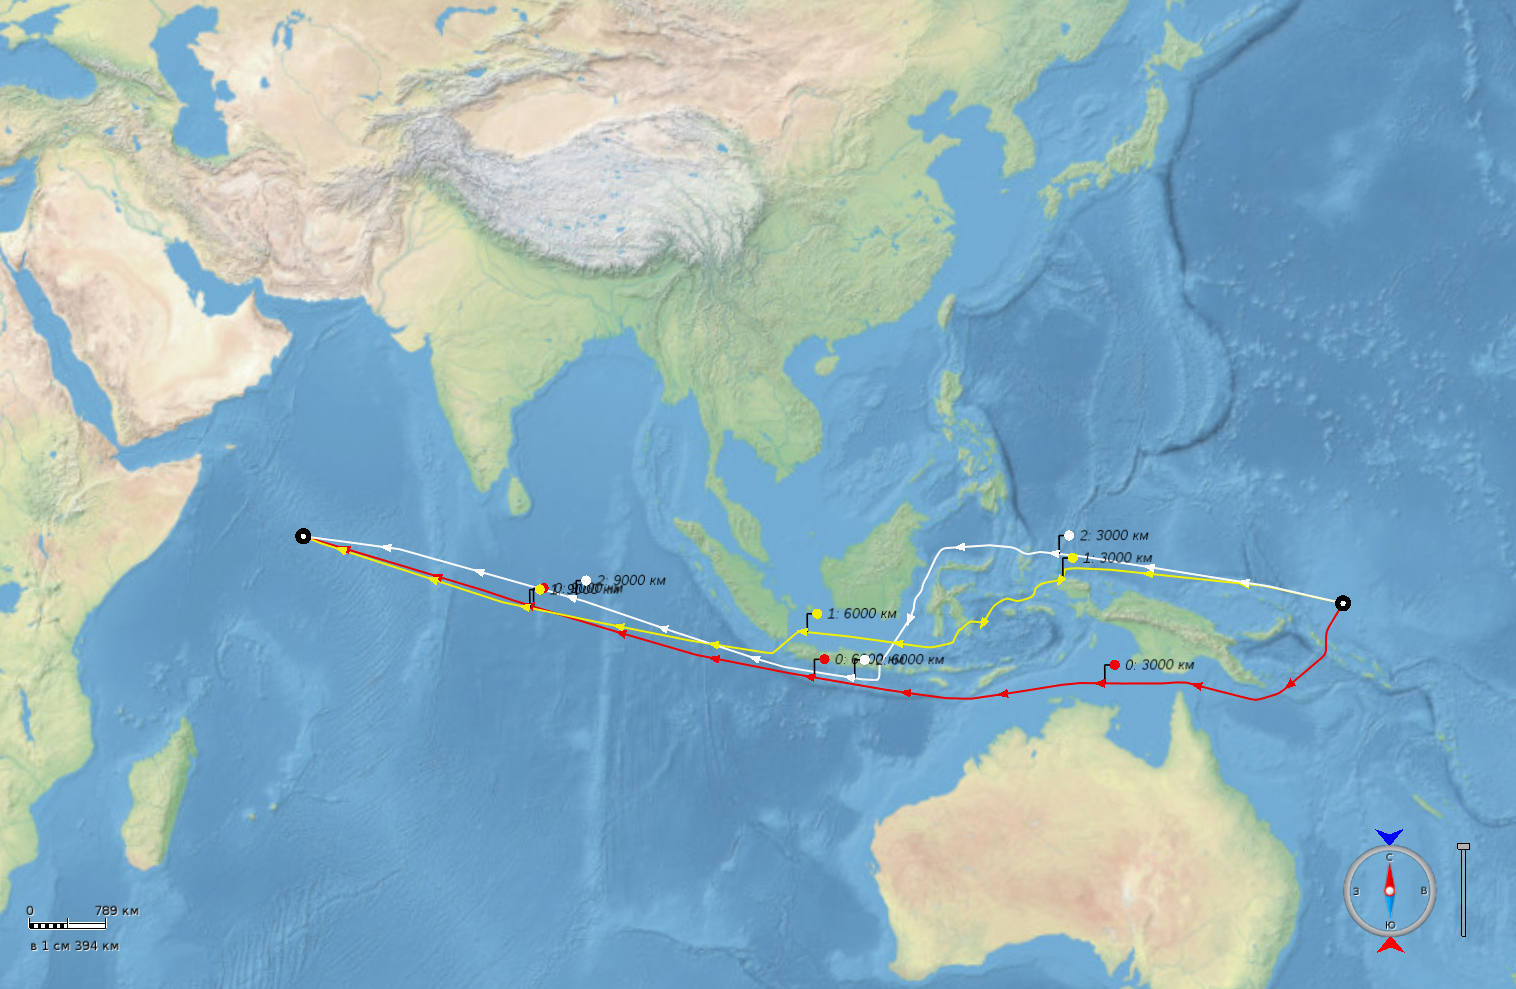
\includegraphics[width=\textwidth]{Results/comparison/bad2}
    \caption{Найдены похожие маршруты}
    \label{fig:res-comp-bad2}
\end{figure}

\begin{figure}
    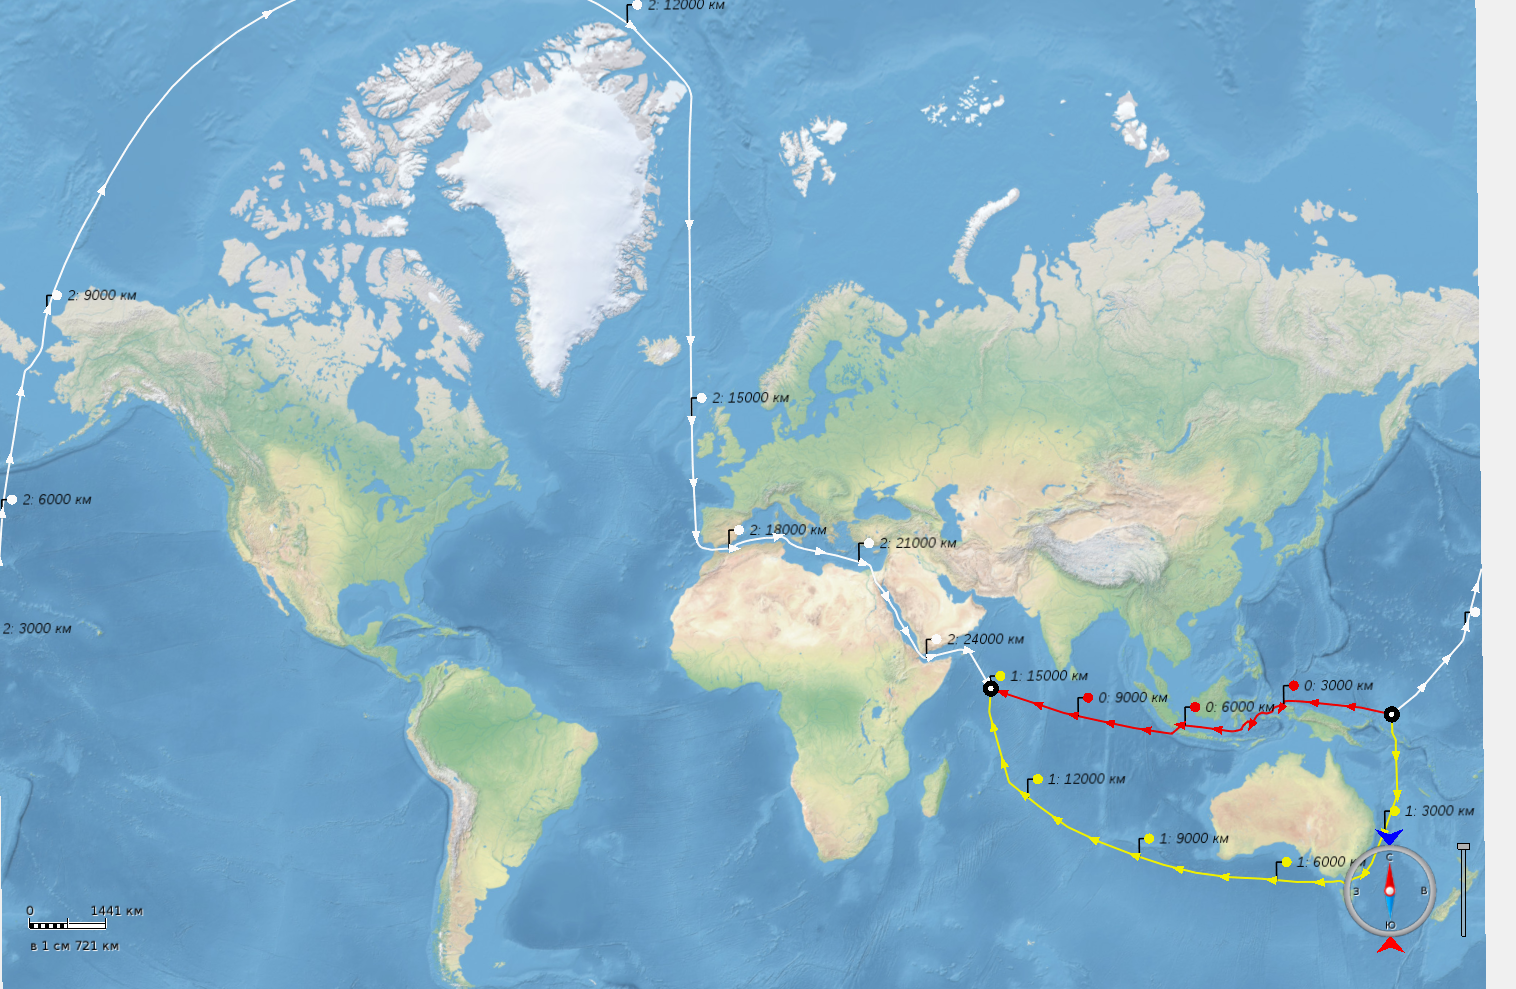
\includegraphics[width=\textwidth]{Results/comparison/good2}
    \caption{Найдены маршруты с разными способами обхода материков}
    \label{fig:res-comp-good2}
\end{figure}

Для примера проведём сравнение маршрутов, находимых разработанным
алгоритмом, с маршрутами, находимыми
алгоритмом~\cite{lim2005shortest}. На рисунках \ref{fig:res-comp-bad1}
и \ref{fig:res-comp-good1} показана ситуация, в которой алгоритм,
описанный Лимом и Кимом, нашёл лишь один маршрут, а алгоритм,
описанный в данной работе, нашёл три различных маршрута. В ситуации,
показанной на рисунках \ref{fig:res-comp-bad2} и
\ref{fig:res-comp-good2}, оба алгоритма нашли три маршрута. Однако в
первом случае маршруты, не являются существенно различными, хоть и
обходят препятствия разными способами, поскольку размеры этих
препятствий невелики. К тому же найденные маршруты не являются
локально оптимальными, так как в конце пути имеются некоторые
различия. Во втором случае было найдено три существенно разных
маршрута, различающихся способами обхода материков. Таким образом,
показано, что разработанный алгоритм лучше подходит для решения
поставленной задачи, хотя общая идея у них похожа.

В заключение приведём несколько рисунков, демонстрирующих результаты
работы алгоритма на сфере (рис.~\ref{fig:result1}, \ref{fig:result2}).

\begin{figure}
    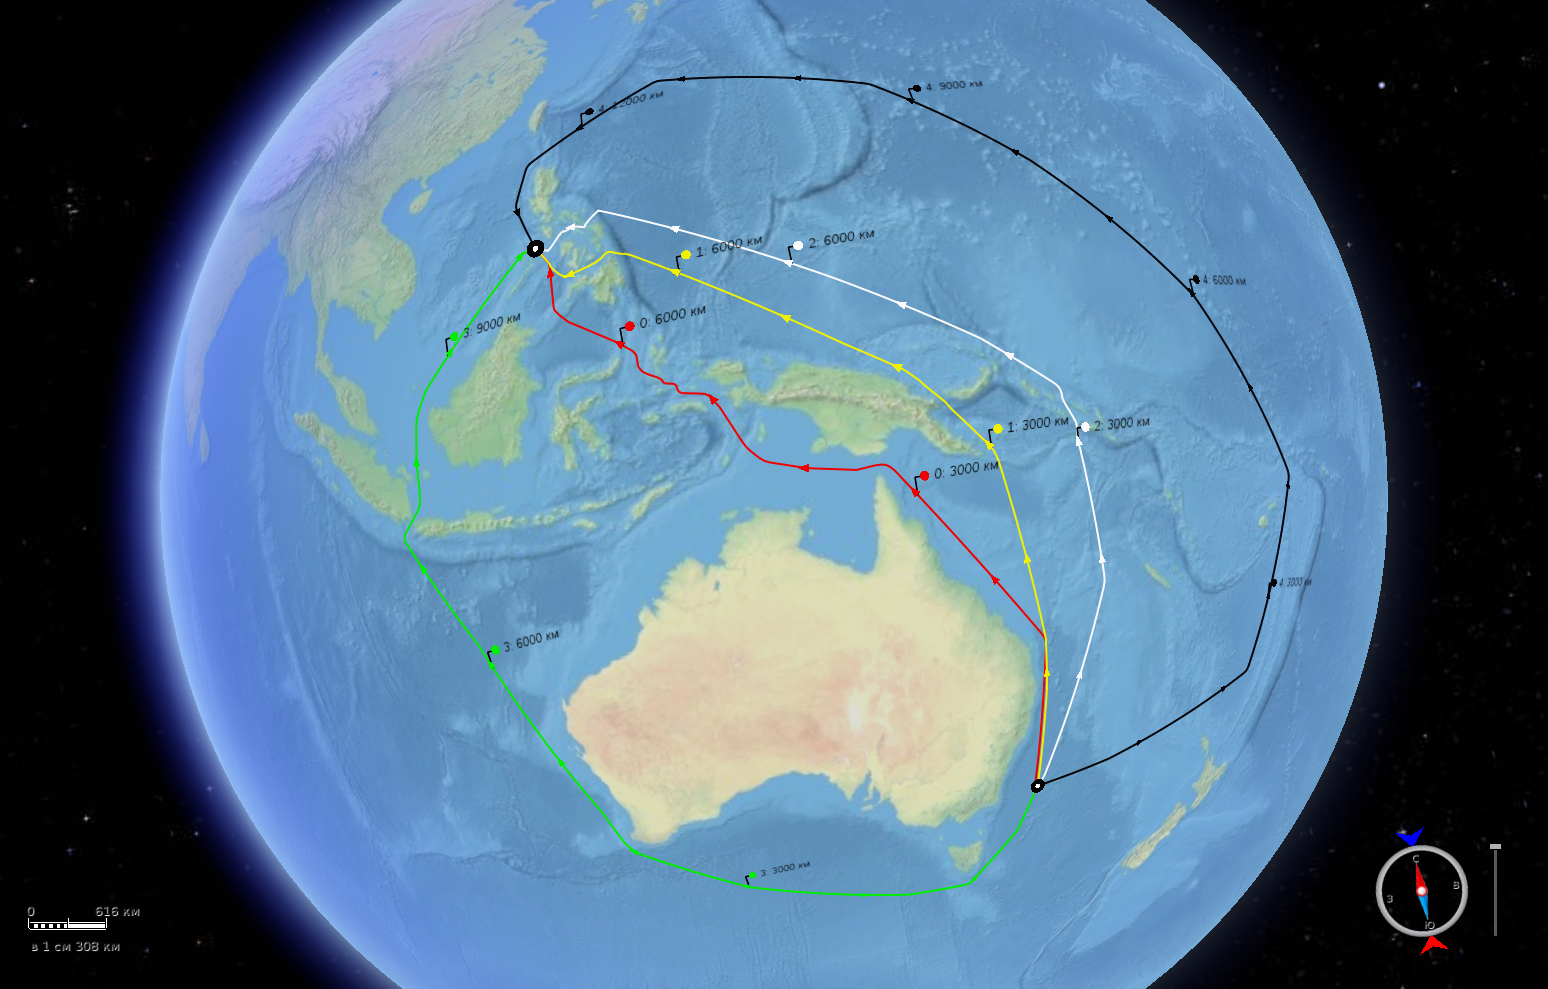
\includegraphics[width=\textwidth]{Results/1}
    \caption{Маршруты на сфере}
    \label{fig:result1}
\end{figure}

\begin{figure}
    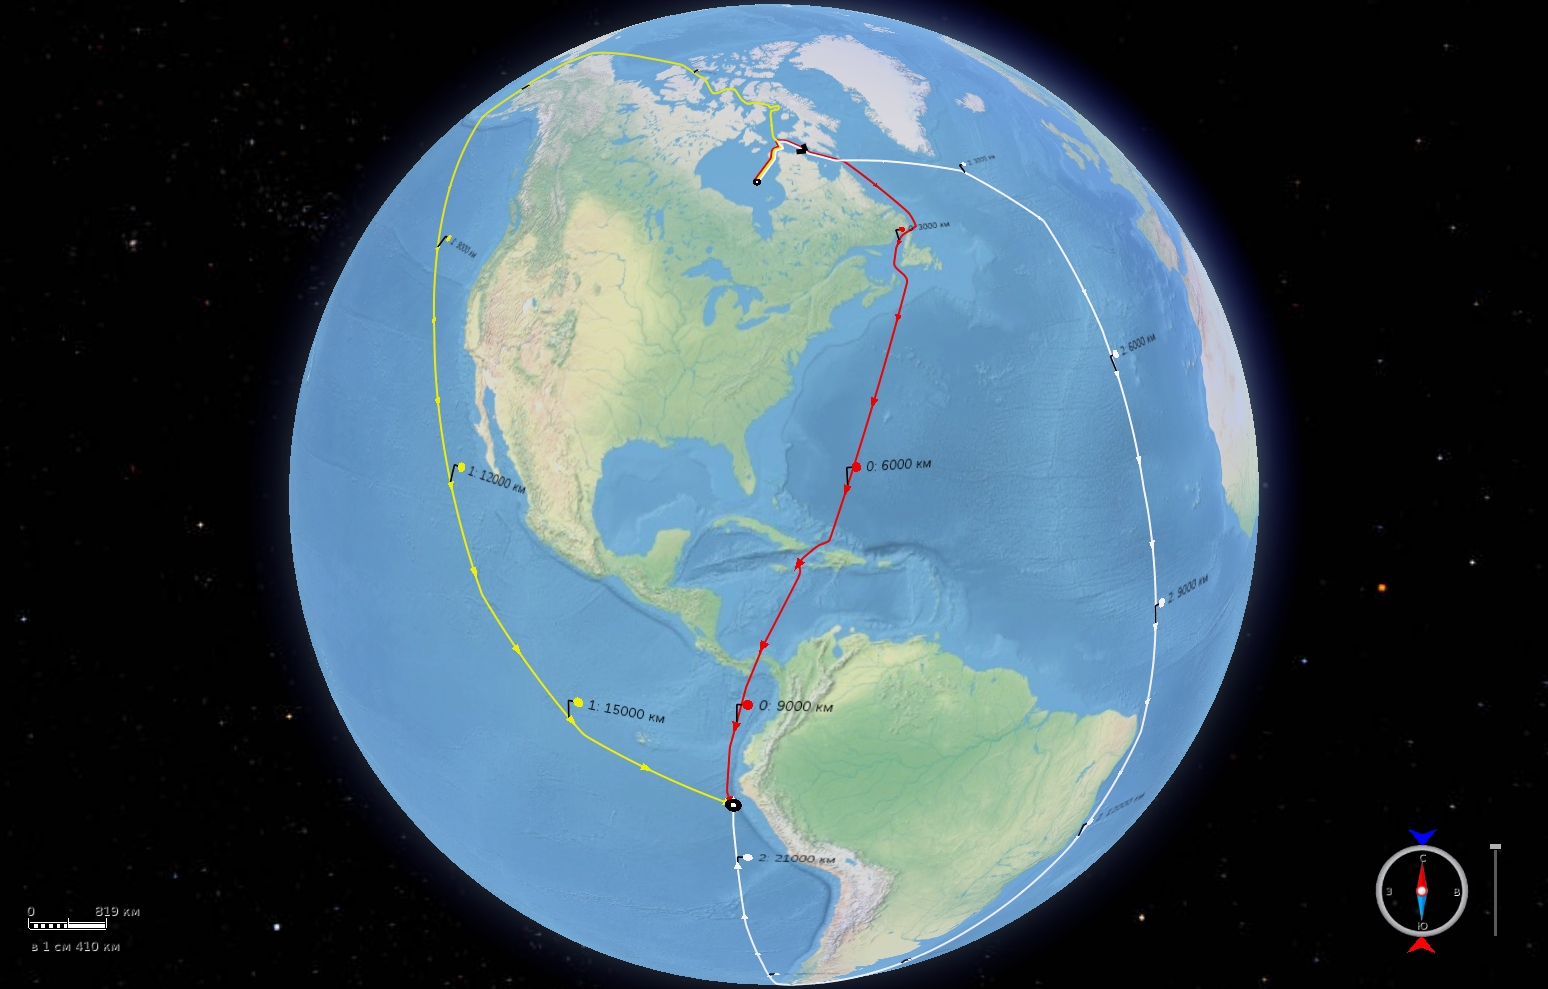
\includegraphics[width=\textwidth]{Results/2}
    \caption{Маршруты на сфере}
    \label{fig:result2}
\end{figure}

\FloatBarrier


\startconclusionpage

Нормально

\FloatBarrier


\printbibliography[heading=trueHeading]

\end{document}

